% Options for packages loaded elsewhere
\PassOptionsToPackage{unicode}{hyperref}
\PassOptionsToPackage{hyphens}{url}
%
\documentclass[
  11pt,
  oneside]{book}
\usepackage{amsmath,amssymb}
\usepackage{iftex}
\ifPDFTeX
  \usepackage[T1]{fontenc}
  \usepackage[utf8]{inputenc}
  \usepackage{textcomp} % provide euro and other symbols
\else % if luatex or xetex
  \usepackage{unicode-math} % this also loads fontspec
  \defaultfontfeatures{Scale=MatchLowercase}
  \defaultfontfeatures[\rmfamily]{Ligatures=TeX,Scale=1}
\fi
\usepackage{lmodern}
\ifPDFTeX\else
  % xetex/luatex font selection
\fi
% Use upquote if available, for straight quotes in verbatim environments
\IfFileExists{upquote.sty}{\usepackage{upquote}}{}
\IfFileExists{microtype.sty}{% use microtype if available
  \usepackage[]{microtype}
  \UseMicrotypeSet[protrusion]{basicmath} % disable protrusion for tt fonts
}{}
\makeatletter
\@ifundefined{KOMAClassName}{% if non-KOMA class
  \IfFileExists{parskip.sty}{%
    \usepackage{parskip}
  }{% else
    \setlength{\parindent}{0pt}
    \setlength{\parskip}{6pt plus 2pt minus 1pt}}
}{% if KOMA class
  \KOMAoptions{parskip=half}}
\makeatother
\usepackage{xcolor}
\usepackage[margin=1in]{geometry}
\usepackage{color}
\usepackage{fancyvrb}
\newcommand{\VerbBar}{|}
\newcommand{\VERB}{\Verb[commandchars=\\\{\}]}
\DefineVerbatimEnvironment{Highlighting}{Verbatim}{commandchars=\\\{\}}
% Add ',fontsize=\small' for more characters per line
\usepackage{framed}
\definecolor{shadecolor}{RGB}{248,248,248}
\newenvironment{Shaded}{\begin{snugshade}}{\end{snugshade}}
\newcommand{\AlertTok}[1]{\textcolor[rgb]{0.94,0.16,0.16}{#1}}
\newcommand{\AnnotationTok}[1]{\textcolor[rgb]{0.56,0.35,0.01}{\textbf{\textit{#1}}}}
\newcommand{\AttributeTok}[1]{\textcolor[rgb]{0.13,0.29,0.53}{#1}}
\newcommand{\BaseNTok}[1]{\textcolor[rgb]{0.00,0.00,0.81}{#1}}
\newcommand{\BuiltInTok}[1]{#1}
\newcommand{\CharTok}[1]{\textcolor[rgb]{0.31,0.60,0.02}{#1}}
\newcommand{\CommentTok}[1]{\textcolor[rgb]{0.56,0.35,0.01}{\textit{#1}}}
\newcommand{\CommentVarTok}[1]{\textcolor[rgb]{0.56,0.35,0.01}{\textbf{\textit{#1}}}}
\newcommand{\ConstantTok}[1]{\textcolor[rgb]{0.56,0.35,0.01}{#1}}
\newcommand{\ControlFlowTok}[1]{\textcolor[rgb]{0.13,0.29,0.53}{\textbf{#1}}}
\newcommand{\DataTypeTok}[1]{\textcolor[rgb]{0.13,0.29,0.53}{#1}}
\newcommand{\DecValTok}[1]{\textcolor[rgb]{0.00,0.00,0.81}{#1}}
\newcommand{\DocumentationTok}[1]{\textcolor[rgb]{0.56,0.35,0.01}{\textbf{\textit{#1}}}}
\newcommand{\ErrorTok}[1]{\textcolor[rgb]{0.64,0.00,0.00}{\textbf{#1}}}
\newcommand{\ExtensionTok}[1]{#1}
\newcommand{\FloatTok}[1]{\textcolor[rgb]{0.00,0.00,0.81}{#1}}
\newcommand{\FunctionTok}[1]{\textcolor[rgb]{0.13,0.29,0.53}{\textbf{#1}}}
\newcommand{\ImportTok}[1]{#1}
\newcommand{\InformationTok}[1]{\textcolor[rgb]{0.56,0.35,0.01}{\textbf{\textit{#1}}}}
\newcommand{\KeywordTok}[1]{\textcolor[rgb]{0.13,0.29,0.53}{\textbf{#1}}}
\newcommand{\NormalTok}[1]{#1}
\newcommand{\OperatorTok}[1]{\textcolor[rgb]{0.81,0.36,0.00}{\textbf{#1}}}
\newcommand{\OtherTok}[1]{\textcolor[rgb]{0.56,0.35,0.01}{#1}}
\newcommand{\PreprocessorTok}[1]{\textcolor[rgb]{0.56,0.35,0.01}{\textit{#1}}}
\newcommand{\RegionMarkerTok}[1]{#1}
\newcommand{\SpecialCharTok}[1]{\textcolor[rgb]{0.81,0.36,0.00}{\textbf{#1}}}
\newcommand{\SpecialStringTok}[1]{\textcolor[rgb]{0.31,0.60,0.02}{#1}}
\newcommand{\StringTok}[1]{\textcolor[rgb]{0.31,0.60,0.02}{#1}}
\newcommand{\VariableTok}[1]{\textcolor[rgb]{0.00,0.00,0.00}{#1}}
\newcommand{\VerbatimStringTok}[1]{\textcolor[rgb]{0.31,0.60,0.02}{#1}}
\newcommand{\WarningTok}[1]{\textcolor[rgb]{0.56,0.35,0.01}{\textbf{\textit{#1}}}}
\usepackage{longtable,booktabs,array}
\usepackage{calc} % for calculating minipage widths
% Correct order of tables after \paragraph or \subparagraph
\usepackage{etoolbox}
\makeatletter
\patchcmd\longtable{\par}{\if@noskipsec\mbox{}\fi\par}{}{}
\makeatother
% Allow footnotes in longtable head/foot
\IfFileExists{footnotehyper.sty}{\usepackage{footnotehyper}}{\usepackage{footnote}}
\makesavenoteenv{longtable}
\usepackage{graphicx}
\makeatletter
\def\maxwidth{\ifdim\Gin@nat@width>\linewidth\linewidth\else\Gin@nat@width\fi}
\def\maxheight{\ifdim\Gin@nat@height>\textheight\textheight\else\Gin@nat@height\fi}
\makeatother
% Scale images if necessary, so that they will not overflow the page
% margins by default, and it is still possible to overwrite the defaults
% using explicit options in \includegraphics[width, height, ...]{}
\setkeys{Gin}{width=\maxwidth,height=\maxheight,keepaspectratio}
% Set default figure placement to htbp
\makeatletter
\def\fps@figure{htbp}
\makeatother
\setlength{\emergencystretch}{3em} % prevent overfull lines
\providecommand{\tightlist}{%
  \setlength{\itemsep}{0pt}\setlength{\parskip}{0pt}}
\setcounter{secnumdepth}{5}
\ifLuaTeX
  \usepackage{selnolig}  % disable illegal ligatures
\fi
\usepackage{bookmark}
\IfFileExists{xurl.sty}{\usepackage{xurl}}{} % add URL line breaks if available
\urlstyle{same}
\hypersetup{
  pdftitle={Notes on Economics},
  pdfauthor={Noushin Nabavi},
  hidelinks,
  pdfcreator={LaTeX via pandoc}}

\title{Notes on Economics}
\author{Noushin Nabavi}
\date{2026-05-24}

\begin{document}
\maketitle

{
\setcounter{tocdepth}{1}
\tableofcontents
}
\chapter{Welcome}\label{welcome}

These notes provide an applied introduction to economics and econometrics, with an emphasis on understanding real-world economic issues and evaluating policy interventions. The material combines economic reasoning with empirical tools commonly used in public policy, health economics, and applied social science.

The focus throughout is on interpretation and judgment rather than formal derivation. Economic models and statistical methods are treated as tools for reasoning about evidence rather than as ends in themselves.

\section{Who this book is for}\label{who-this-book-is-for}

These notes are intended for students in economics, public policy, health sciences, and related fields, as well as analysts and researchers working with applied economic data. The material is also suitable for readers with basic quantitative literacy who want to understand how economic evidence is produced and interpreted.

The book does not assume advanced mathematics. Familiarity with introductory statistics is helpful, but not required for all chapters.

\section{How the book is organized}\label{how-the-book-is-organized}

The chapters progress from concepts to methods to applications.

Early sections introduce economic thinking, scarcity, incentives, institutions, and market structure. Middle sections develop core microeconomic and macroeconomic ideas, including stabilization policy and economic measurement. Later sections focus on empirical methods such as regression, time-series analysis, and quasi-experimental approaches used in policy evaluation.

Although chapters are designed to be readable independently, later material builds on ideas introduced earlier in the book.

\section{Using figures and visuals}\label{using-figures-and-visuals}

Figures are used throughout the book to support intuition before formal models or code are introduced. Visualizations help clarify relationships between economic actors and variables, illustrate dynamic patterns such as trends and interventions, and support interpretation of statistical results.

Figures are referenced directly in the text and are intended to function as conceptual anchors that readers can revisit while working through later chapters.

\section{Using R code}\label{using-r-code}

Some chapters include R code to demonstrate empirical workflows commonly used in applied economics and policy analysis.

Code chunks are included primarily as examples and templates. Some chunks may use \texttt{eval\ =\ FALSE} so the book can render without requiring all packages or datasets. Readers who wish to run the code locally can enable evaluation after installing the necessary packages and ensuring data availability.

The emphasis is on understanding the logic of analysis and interpretation rather than reproducing exact numerical outputs.

\section{Learning goals}\label{learning-goals}

By the end of these notes, readers should be able to:

\begin{itemize}
\tightlist
\item
  explain core economic concepts and relate them to real-world policy questions;
\item
  interpret common economic indicators such as GDP, inflation, and unemployment;
\item
  understand the logic and limitations of regression-based analysis;
\item
  recognize issues of trend, autocorrelation, and stationarity in time-series data; and
\item
  assess policy interventions using quasi-experimental reasoning, including interrupted time series analysis.
\end{itemize}

\section{A note on interpretation and evidence}\label{a-note-on-interpretation-and-evidence}

Economic and statistical models simplify reality. Throughout the book, emphasis is placed not only on estimation and prediction, but also on interpretation, assumptions, uncertainty, and institutional context.

Economic evidence is always produced within data, measurement, and modeling constraints. Readers are encouraged to approach results critically, paying attention to the assumptions underlying models and the limitations of available evidence.

The goal of the book is not to present economic analysis as a mechanical procedure, but rather as a structured framework for reasoning about complex real-world problems.

\chapter{What is Economics?}\label{what-is-econ}

Economics studies how individuals, organizations, and governments make choices under conditions of scarcity. Because resources are limited, every choice involves trade-offs. These trade-offs are shaped not only by prices and resources, but also by institutions, incentives, information, social norms, and power.

Economics is therefore not only about money or markets. It is also about how societies organize production, distribute resources, manage risk, and define what counts as a desirable outcome. Questions about housing affordability, healthcare access, environmental degradation, taxation, inflation, and climate policy are all economic questions because they involve competing objectives under limited resources.

For example, during a drought, water may need to be allocated among households, agriculture, ecosystems, and industry. Economics helps analyze who receives water, who bears the costs, what incentives exist, and how institutions shape the outcome.

This chapter introduces core concepts and vocabulary used throughout the rest of the book.

\section{Roadmap}\label{roadmap}

The chapter begins with scarcity and opportunity cost, then introduces the role of incentives, values, institutions, and information in economic reasoning. It next examines economic actors and market structures before concluding with market failure and the role of policy evaluation.

\section{Learning objectives}\label{learning-objectives}

By the end of this chapter, you should be able to:

\begin{itemize}
\tightlist
\item
  define scarcity, opportunity cost, and incentives;
\item
  explain why economic evaluation involves both evidence and values;
\item
  compare broad economic traditions and their assumptions;
\item
  identify major economic actors and explain how their objectives differ; and
\item
  explain why market failures matter in applied policy analysis.
\end{itemize}

\begin{figure}

{\centering 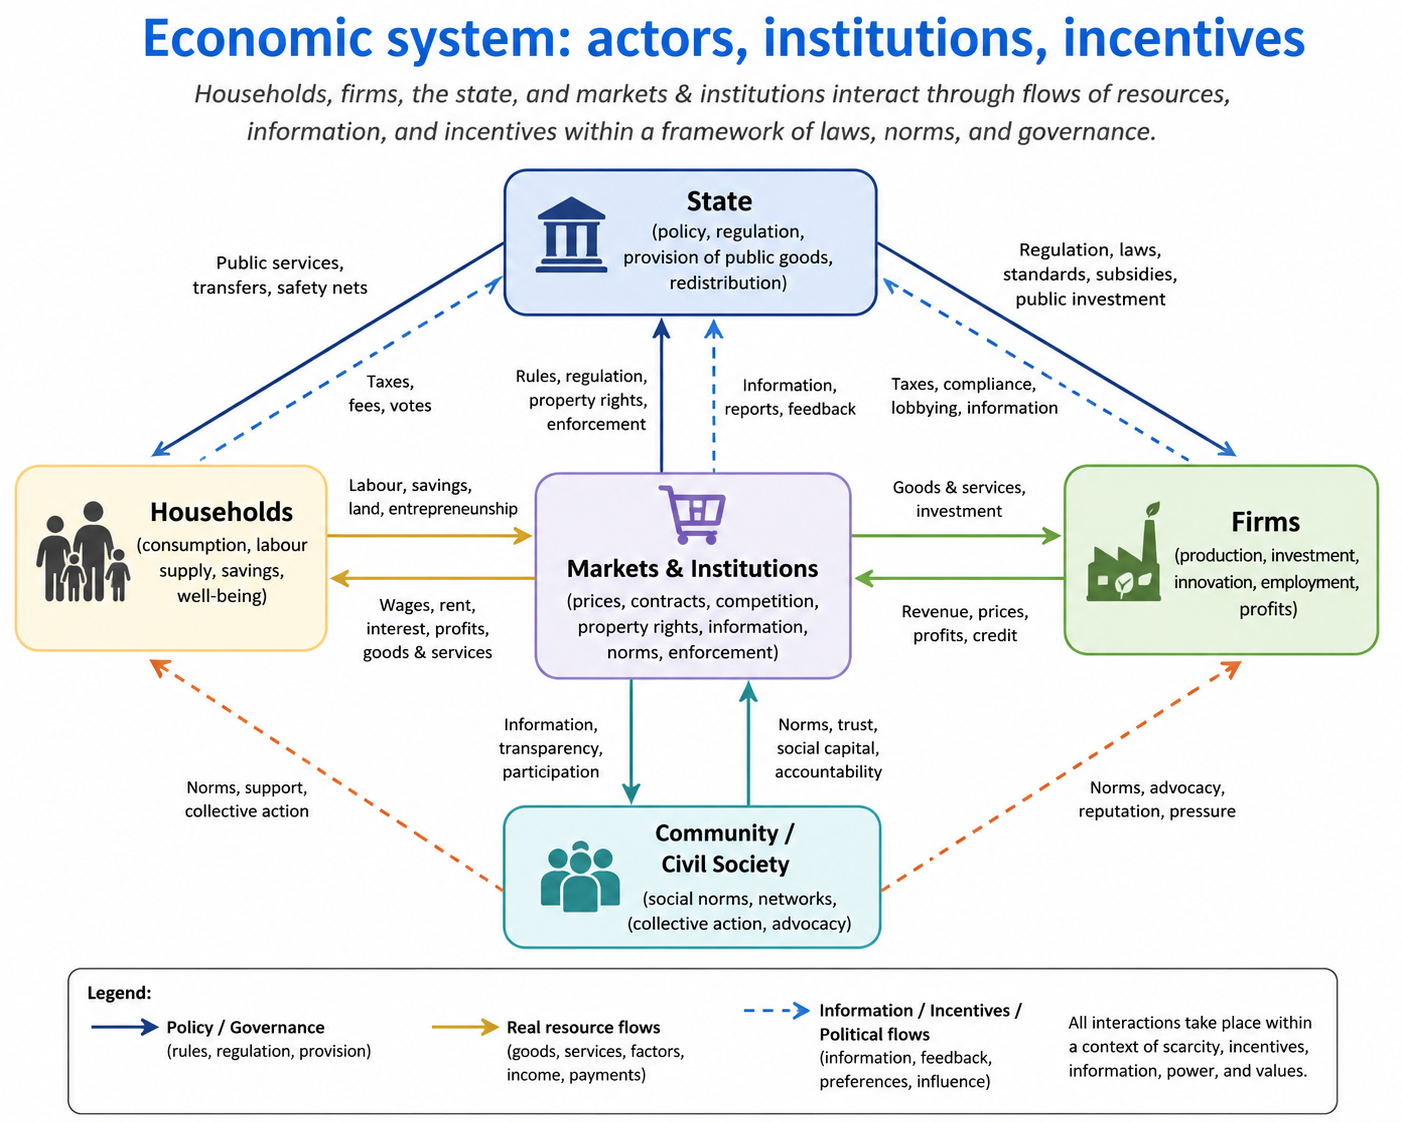
\includegraphics[width=1\linewidth]{images/01_econ_system_map} 

}

\caption{Economic system overview showing households, firms, markets and institutions, the state, and civil society. The diagram highlights flows of resources, incentives, information, regulation, and power within the economy.}\label{fig:fig-econ-system}
\end{figure}

Figure \ref{fig:fig-econ-system} presents a high-level view of the economic system. The figure is not a mathematical model. Instead, it is a conceptual map showing how economic actors interact through flows of labour, goods, services, taxes, regulation, information, incentives, and social norms.

The figure also emphasizes that markets do not operate in isolation. Economic activity occurs within broader institutional systems that include laws, governance structures, political systems, and cultural norms. In applied economics, disagreements often arise because people make different assumptions about which relationships are most important, which actors hold power, and which constraints matter most.

\section{Scarcity, trade-offs, and opportunity cost}\label{scarcity-trade-offs-and-opportunity-cost}

Scarcity means that resources are limited relative to human wants and needs. These resources include money, labour, time, land, energy, institutional capacity, public budgets, and even attention.

Because resources are limited, choices must be made. Choosing one option usually means giving up another. This forgone alternative is called the \emph{opportunity cost}.

For example, spending public funds on transportation infrastructure may reduce the funding available for healthcare or education. Protecting environmentally sensitive land may reduce opportunities for industrial development or resource extraction. Similarly, a student who spends time studying gives up leisure time or paid employment.

Opportunity costs are not always monetary. In policy contexts, they may include environmental degradation, reduced trust, poorer health outcomes, or lost social opportunities.

In applied economic analysis, opportunity cost is often evaluated by comparing a world \emph{with} an intervention to a world \emph{without} it. This comparison is called a \emph{counterfactual}, and it becomes central later in the book.

\section{Incentives and behaviour}\label{incentives-and-behaviour}

Incentives influence how individuals and organizations respond to policies, prices, risks, and information. Incentives may be financial, legal, social, political, or psychological.

For example, taxes on pollution attempt to discourage environmentally harmful activities, while subsidies for renewable energy attempt to encourage cleaner forms of production. Wage levels influence labour supply decisions, and social recognition may encourage volunteering or cooperation.

Economists often study how changes in incentives alter behaviour. However, incentives do not operate independently from social systems. Behaviour is also shaped by institutions, culture, laws, information, and unequal power relationships.

\section{Economics as evidence and as judgment}\label{economics-as-evidence-and-as-judgment}

Economics uses evidence, data, and models to explain patterns and evaluate decisions. At the same time, economics also involves judgments about what outcomes are desirable.

One common criterion is \emph{efficiency}, although efficiency can be interpreted in different ways. A narrow interpretation focuses on maximizing outputs for a given set of inputs. Broader interpretations may include long-term sustainability, resilience, spillover effects, and system-wide impacts.

Economic evaluation also involves values such as fairness, equality, freedom, stability, and environmental sustainability. Many policy debates are ultimately disagreements about which values should receive priority and what trade-offs are considered acceptable.

For example, a policy may increase total economic output while simultaneously increasing inequality. In such cases, disagreements are often not about the evidence itself, but about how outcomes should be evaluated.

\section{Economic theories and assumptions}\label{economic-theories-and-assumptions}

Different economic traditions emphasize different mechanisms and assumptions.

Neoclassical economics often begins with simplified models of competitive markets, rational decision-making, and price-driven coordination. These models are useful because they provide clear analytical frameworks and benchmarks for comparison. However, real-world economies frequently depart from these idealized assumptions.

Institutional and social approaches emphasize that markets are embedded within legal systems, political structures, social norms, and historical relationships. From this perspective, property rights, governance systems, trust, and power are central parts of economic analysis rather than background conditions.

Post-Keynesian approaches place greater emphasis on uncertainty, instability, financial systems, market power, and effective demand. These perspectives often argue that economies do not naturally move toward stable equilibrium and may require active policy intervention.

Economic theories also differ in how they treat information. Some approaches rely on simplified assumptions where actors possess relatively complete information and markets can be analyzed using formal models. Other approaches emphasize uncertainty, incomplete information, bounded rationality, and social complexity.

These differences matter because policy conclusions often depend heavily on assumptions about behaviour, information, and institutions.

\section{Economic actors}\label{economic-actors}

Economic systems involve multiple actors with different objectives and constraints. Figure \ref{fig:fig-econ-system} highlights how these actors interact through flows of resources, information, incentives, regulation, and social influence.

Households supply labour, consume goods and services, save, borrow, and make decisions under uncertainty. Households are rarely a single unified decision-maker. Bargaining, caregiving responsibilities, unequal income distribution, and risk-sharing arrangements within households can affect labour supply, education, consumption, and health outcomes.

Firms produce goods and services using labour, capital, technology, and natural resources. Although profit is often important, firms may also pursue market share, long-term stability, innovation, political influence, or stakeholder objectives.

Governments influence economic activity through taxation, regulation, public services, infrastructure investment, redistribution, and legal enforcement. The state also shapes markets by defining property rights, enforcing contracts, and responding to market failures.

Community organizations, non-profit groups, Indigenous governments, cooperatives, advocacy groups, and social networks also play important economic roles. These actors can provide mutual aid, influence norms, advocate for policy change, stabilize communities, and build social trust.

\section{Markets and market structure}\label{markets-and-market-structure}

Markets coordinate exchanges between buyers and sellers. However, markets differ greatly in structure, competitiveness, and power distribution.

Perfect competition assumes many buyers and sellers, relatively complete information, and free entry and exit. It is primarily a theoretical benchmark used to organize economic reasoning, even though real-world markets rarely meet all of these conditions.

A monopoly exists when a single seller dominates a market, while a monopsony occurs when a single buyer holds substantial market power. Oligopolies involve a small number of large firms whose decisions affect one another strategically. Monopolistic competition is common in differentiated goods and services where many firms compete but products are not identical.

Market structure is not only about prices and efficiency. It is also about bargaining power, political influence, innovation, and who has control over economic outcomes.

\section{Market failure and why it matters}\label{market-failure-and-why-it-matters}

Market failures occur when markets alone do not produce socially desirable outcomes.

One common example is \emph{externalities}, where actions impose costs or benefits on others that are not reflected in market prices. Pollution and climate change are examples of negative externalities, while vaccination programs may generate positive externalities.

Another example involves \emph{public goods}, which are difficult to exclude people from using and are often underprovided by markets. Examples include flood protection, national defense, and some forms of public health infrastructure.

Markets may also function poorly when one side possesses more information than another. These information problems are common in healthcare, insurance, and financial systems. Concentrated market power can also reduce competition, distort prices, limit innovation, and increase inequality.

Some socially valuable goods or risks may lack functioning markets altogether. Ecosystem services, biodiversity protection, and unpaid caregiving work are examples of activities that are often difficult to measure or price adequately within conventional markets.

Many policy questions arise precisely because markets do not automatically generate equitable, efficient, or sustainable outcomes.

\section{Common pitfalls}\label{common-pitfalls}

A common mistake in economic analysis is treating efficiency as the only policy objective while ignoring equity and distributional impacts. Another is assuming that markets are competitive when significant market power exists. Analysts may also overlook the importance of institutions, governance systems, historical context, or unequal bargaining power.

Narrow cost-benefit frameworks can become misleading when important social or environmental impacts are difficult to measure. Similarly, treating households and communities as passive background conditions rather than active economic actors can lead to incomplete analysis.

\section{Key takeaways}\label{key-takeaways}

Economics studies how societies make choices under scarcity and how those choices create trade-offs. Economic outcomes are shaped not only by prices and resources, but also by institutions, incentives, information, and power.

Markets operate within broader political, legal, and social systems, and market structure strongly influences efficiency, bargaining power, and policy outcomes. Because markets do not always produce socially desirable results, governments and institutions often intervene to address market failures and broader social objectives.

\chapter{Microeconomics Essentials}\label{micro}

Microeconomics studies how individuals, households, firms, and governments make decisions and interact within markets. It explains how prices and quantities emerge, how incentives shape behaviour, and how policies affect economic outcomes. Many of the tools introduced in this chapter are widely used in applied policy analysis, including healthcare, environmental regulation, labour markets, taxation, and public infrastructure planning.

For example, when governments introduce a carbon tax, regulate rental housing, subsidize public transit, or impose tariffs, economists analyze how consumers and firms respond, how prices and production change, and who ultimately bears the costs and benefits. Microeconomics provides the conceptual tools for understanding these behavioural and policy effects.

This chapter begins with supply and demand as a framework for understanding market equilibrium. It then introduces welfare, elasticity, and tax incidence before connecting market structure to market power. The chapter concludes with externalities and public goods as major reasons why governments and institutions intervene in markets.

\section{Learning objectives}\label{learning-objectives-1}

By the end of this chapter, you should be able to:

\begin{itemize}
\tightlist
\item
  explain how supply and demand determine equilibrium prices and quantities;
\item
  interpret elasticity and connect it to behavioural response;
\item
  explain economic incidence and why policy burdens do not always fall where policies are legally applied;
\item
  describe how market power emerges and how governments attempt to regulate it; and
\item
  explain why externalities and public goods can lead to market failure.
\end{itemize}

\begin{figure}

{\centering 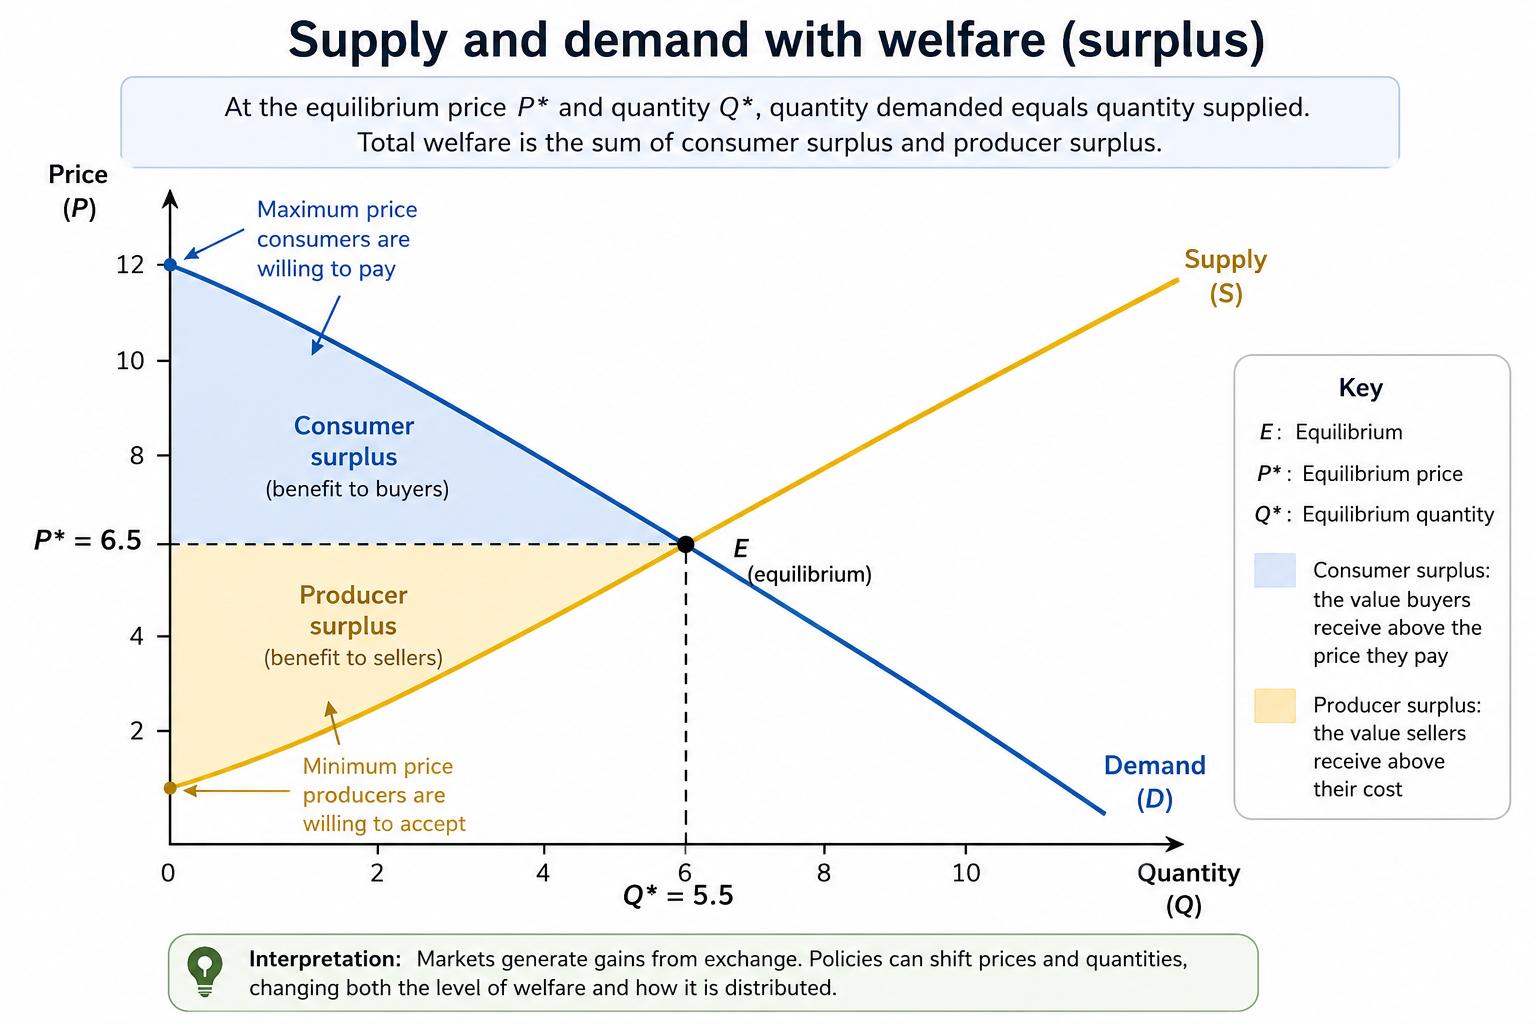
\includegraphics[width=1\linewidth]{images/02_supply_demand_surplus} 

}

\caption{Supply and demand with welfare areas. Consumer surplus represents the value buyers receive above the market price, while producer surplus represents the value sellers receive above their costs. The figure highlights how policies can affect not only prices and quantities, but also the distribution of welfare.}\label{fig:fig-sd-surplus}
\end{figure}

Figure \ref{fig:fig-sd-surplus} illustrates one of the most important ideas in microeconomics: markets generate gains from exchange. The equilibrium point occurs where quantity demanded equals quantity supplied. At this point, both buyers and sellers benefit from participating in the market.

The shaded areas in the figure represent \emph{consumer surplus} and \emph{producer surplus}. Consumer surplus measures the difference between what consumers are willing to pay and what they actually pay in the market. Producer surplus measures the difference between the market price and the minimum amount producers are willing to accept. Economists often use these concepts as simplified measures of welfare when evaluating policies and market outcomes.

Importantly, economists are often interested in more than equilibrium alone. Public policies can shift prices, quantities, and the distribution of gains and losses across groups. As a result, understanding welfare and incidence is central to applied policy analysis.

\section{Supply, demand, and equilibrium}\label{supply-demand-and-equilibrium}

Demand describes how the quantity demanded of a good or service changes with price, holding other factors constant. In general, consumers purchase more when prices are lower and less when prices are higher. Supply describes how quantity supplied changes with price. Producers are usually willing to supply more when prices increase because production becomes more profitable.

Equilibrium occurs where supply equals demand. At the equilibrium price, the quantity consumers wish to purchase matches the quantity firms wish to sell. Figure \ref{fig:fig-sd-surplus} shows this equilibrium at point \(E\), with equilibrium price \(P^*\) and equilibrium quantity \(Q^*\).

Economists often use \emph{comparative statics} to study how equilibrium changes when market conditions shift. Demand may shift because of changes in income, preferences, population, expectations, or the prices of related goods. Supply may shift because of changes in technology, input costs, taxes, regulation, or environmental conditions.

For example, a drought may reduce agricultural supply, increasing food prices. A subsidy for renewable energy may increase supply by lowering production costs. A rise in consumer income may increase demand for travel, housing, or recreation.

Equilibrium analysis provides a useful starting point for understanding how markets respond to change. However, equilibrium alone does not determine whether outcomes are efficient, equitable, or socially desirable.

\section{Elasticity, behavioural response, and incidence}\label{elasticity-behavioural-response-and-incidence}

Elasticity measures responsiveness. Price elasticity of demand measures the percentage change in quantity demanded resulting from a one percent change in price. Supply elasticity is defined similarly for producers.

Elasticity matters because individuals and firms do not all respond to price changes in the same way. Some goods have relatively \emph{inelastic} demand, meaning consumers change their behaviour only slightly when prices change. Other goods have more \emph{elastic} demand, meaning consumers respond strongly to price increases or decreases.

For example, gasoline demand is often relatively inelastic in the short run because consumers may have limited immediate alternatives. In contrast, demand for luxury goods or vacation travel is often more elastic because purchases can be delayed or substituted more easily.

Elasticity is especially important for understanding \emph{economic incidence}, or who ultimately bears the burden of taxes and policies. The legal responsibility for paying a tax does not necessarily determine who experiences the economic burden.

When demand is relatively inelastic, consumers tend to bear a larger share of a tax because they continue purchasing even when prices rise. When supply is relatively inelastic, producers bear more of the burden because they cannot easily reduce production.

\begin{center}
\includegraphics{notes-on-economics_files/figure-latex/incidence-mini-sim-1} \end{center}

The figure above illustrates this intuition. A steeper demand curve represents more inelastic demand, meaning consumers are less responsive to price changes. In these situations, consumers generally absorb a larger share of taxes or price increases.

Elasticities are also context-dependent and may change over time. Consumers and firms often become more responsive in the long run as they adapt, discover substitutes, or change technologies.

\section{Market power and regulation}\label{market-power-and-regulation}

Perfectly competitive markets are useful analytical benchmarks, but many real-world markets contain significant concentrations of power. Market power exists when firms or buyers can influence prices, wages, output, or market conditions.

Several factors can contribute to market power, including barriers to entry, economies of scale, control over infrastructure, intellectual property, network effects, and access to information. In digital markets, large platforms may become dominant because the value of the platform increases as more users join.

Market power can exist on both the seller and buyer side of markets. Monopoly refers to a market dominated by a single seller, while monopsony refers to a market dominated by a powerful buyer, such as a major employer in a small labour market.

Governments and institutions attempt to address market power through tools such as antitrust law, regulation, procurement design, transparency requirements, price controls, and benchmarking. In public services, market design choices can strongly influence outcomes. Decisions about who can bid, how contracts are structured, and how quality is monitored may be as important as formal regulation itself.

Market structure is therefore not only about prices and efficiency. It is also about bargaining power, access, innovation, political influence, and the distribution of economic gains.

\section{Externalities, public goods, and market failure}\label{externalities-public-goods-and-market-failure}

Markets do not always produce socially desirable outcomes. One important reason is the existence of \emph{externalities}, where actions impose costs or benefits on others that are not reflected in market prices.

Pollution is a common example of a negative externality because firms and consumers may not fully bear the environmental costs of their activities. Climate change is often described as one of the largest negative externalities because many environmental damages are not fully incorporated into market prices. Positive externalities can also exist. Vaccination programs, for example, create benefits for others by reducing disease transmission.

Another important source of market failure involves \emph{public goods}. Public goods are both non-rival and non-excludable, meaning one person's use does not substantially reduce availability to others and people cannot easily be prevented from benefiting. Examples include national defense, flood protection systems, and some forms of public health infrastructure.

Because private decisions often fail to reflect broader social costs and benefits, governments frequently intervene through taxes, subsidies, standards, tradable permits, regulation, or direct public provision. The most appropriate policy tool depends on measurement feasibility, administrative capacity, enforcement, political constraints, and equity considerations.

Understanding market failure is central to policy analysis because many public interventions are motivated by situations where markets alone do not generate efficient, equitable, or sustainable outcomes.

\section{Common pitfalls and key takeaways}\label{common-pitfalls-and-key-takeaways}

Several common misunderstandings appear repeatedly in applied microeconomics. One is treating elasticity as a fixed number rather than something that depends on context, time horizon, and available substitutes. Another is assuming that taxes always generate large behavioural responses or substantial government revenue. Analysts may also overlook quality, enforcement, or access issues when discussing market interventions.

It is equally important to remember that market power can exist on the buyer side as well as the seller side, and that perfectly competitive markets are often theoretical benchmarks rather than realistic descriptions of actual economies.

Overall, microeconomics provides a framework for understanding how incentives shape behaviour, how markets coordinate economic activity, and why governments intervene when markets fail to achieve broader social objectives. Equilibrium analysis is an important starting point, but welfare, incidence, market power, and externalities are often what matter most in real-world policy decisions.

\chapter{Macroeconomics: Measurement and Trends}\label{macro}

Macroeconomics studies the economy as a whole. It focuses on broad economic conditions such as growth, inflation, unemployment, financial stability, and business cycles. Macroeconomics helps explain why economies expand, slow down, experience recessions, or recover from crises. It also examines how economic conditions affect households, firms, governments, and regions differently.

Unlike microeconomics, which studies individual markets and decisions, macroeconomics looks at aggregate outcomes across the economy. Policymakers use macroeconomic indicators to guide decisions about interest rates, taxation, government spending, employment policy, and social programs. However, macroeconomic indicators are imperfect measures. Understanding what they capture---and what they miss---is central to responsible economic interpretation.

This chapter introduces major macroeconomic indicators, including GDP, inflation, and unemployment, and explains how they are measured and interpreted. It then distinguishes long-run economic growth from short-run business cycles before examining why distribution and inequality matter for understanding macroeconomic performance.

\section{Learning objectives}\label{learning-objectives-2}

By the end of this chapter, you should be able to:

\begin{itemize}
\tightlist
\item
  describe what GDP measures and what it does not measure;
\item
  explain how inflation is measured and why price indices can differ;
\item
  interpret unemployment and labour force participation measures;
\item
  distinguish long-run economic growth from short-run business cycles; and
\item
  explain why distribution and inequality matter for macroeconomic interpretation and policy.
\end{itemize}

\begin{figure}

{\centering 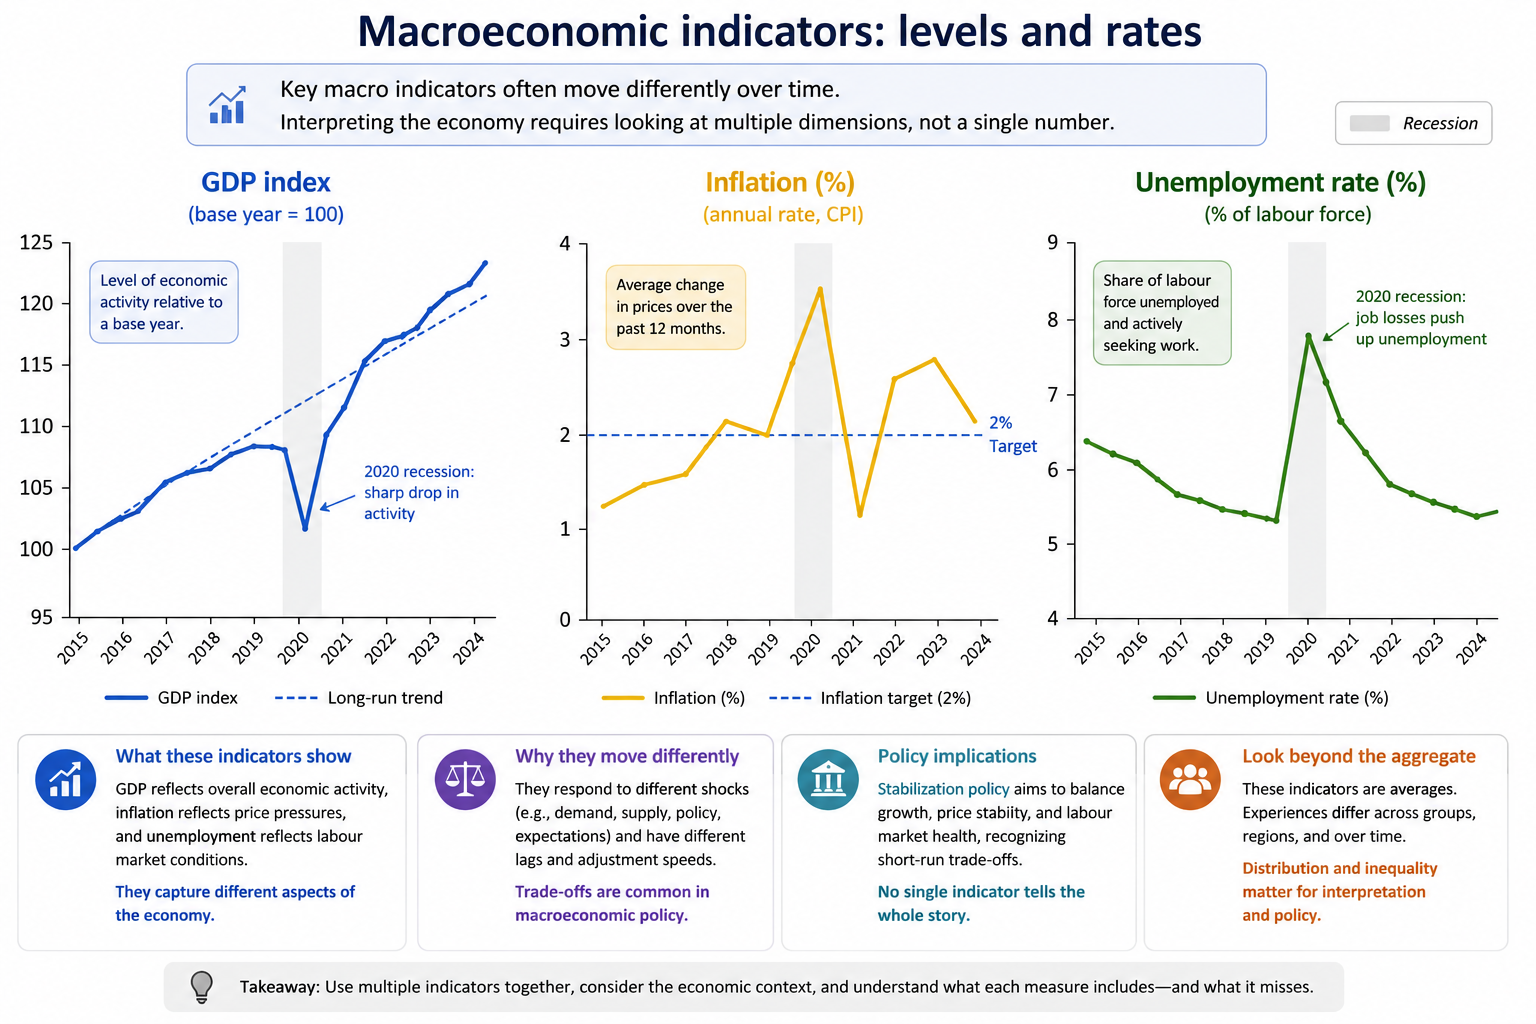
\includegraphics[width=1\linewidth]{images/03_macro_dashboard} 

}

\caption{Illustrative dashboard of macroeconomic indicators. GDP, inflation, and unemployment capture different dimensions of economic conditions and often move differently over time. Recession shading highlights how macroeconomic shocks affect multiple indicators simultaneously.}\label{fig:fig-macro-dashboard}
\end{figure}

Figure \ref{fig:fig-macro-dashboard} presents a simplified macroeconomic dashboard. The figure highlights an important principle in macroeconomics: no single indicator tells the entire story of the economy. Economic growth, inflation, and unemployment often move differently over time, creating trade-offs for policymakers and households.

The figure also illustrates that macroeconomic indicators are connected but not identical. GDP reflects overall economic activity, inflation reflects changes in prices, and unemployment reflects labour market conditions. During recessions, GDP growth may slow or decline while unemployment rises. Inflation may increase, decrease, or remain relatively stable depending on the source of the shock.

Macroeconomic interpretation therefore requires examining multiple indicators together rather than relying on a single measure.

\section{GDP, economic activity, and national accounts}\label{gdp-economic-activity-and-national-accounts}

Gross Domestic Product (GDP) measures the value of final goods and services produced within a country over a given period. GDP is widely used because it provides a broad indicator of economic activity and allows comparisons across time and countries.

Economists often distinguish between \emph{nominal GDP} and \emph{real GDP}. Nominal GDP is measured using current market prices, while real GDP adjusts for inflation. Real GDP is generally more useful for analyzing changes in production and living standards over time because it removes the effects of changing prices.

GDP per capita is also commonly used as a rough measure of average living standards. However, GDP and GDP per capita are not measures of overall well-being. They capture market activity, but they do not fully reflect quality of life, environmental sustainability, inequality, unpaid labour, or social conditions.

For example, unpaid caregiving and household work contribute substantially to society but are often excluded from GDP because no market transaction occurs. Similarly, environmental degradation may accompany rising GDP even when long-term ecological conditions worsen.

GDP can also become difficult to interpret after disasters or economic shocks. Rebuilding after floods, fires, or wars may increase measured economic activity even though overall welfare has declined.

As a result, GDP is best understood as a measure of economic production rather than a complete measure of social progress.

\section{Inflation, prices, and purchasing power}\label{inflation-prices-and-purchasing-power}

Inflation measures the average change in prices over time. The Consumer Price Index (CPI) is one of the most commonly used inflation measures and is based on the cost of a representative basket of goods and services purchased by households.

However, inflation measurement involves important methodological choices. Inflation estimates depend on the composition of the consumption basket, substitution between goods, quality adjustments, and the treatment of housing and other major expenses.

Different households may therefore experience inflation differently. For example, rising housing or food costs may affect low-income households more severely because these expenses represent a larger share of their budgets.

Inflation is not simply a statistical measure; it affects purchasing power, wages, savings, borrowing, investment decisions, and distributional outcomes. Moderate inflation is often considered manageable, but high or unstable inflation can create uncertainty and redistribute resources unpredictably across groups.

At the same time, reducing inflation too aggressively may slow economic activity and increase unemployment depending on economic conditions. Central banks therefore often attempt to balance price stability with broader macroeconomic objectives.

In Figure \ref{fig:fig-macro-dashboard}, the dashed line in the inflation panel represents a typical inflation target. Inflation fluctuates around this target over time, reflecting changing economic conditions, supply disruptions, policy responses, and expectations.

\section{Unemployment, participation, and labour markets}\label{unemployment-participation-and-labour-markets}

Unemployment measures the share of the labour force that is without work but actively searching for employment. Although widely used, unemployment statistics depend heavily on definitions and measurement choices.

A person who stops actively searching for work may no longer be counted as unemployed even if labour market conditions remain weak. Labour force participation can also change because of retirement, education, caregiving responsibilities, discouragement, illness, or demographic shifts.

For this reason, economists often examine several labour market indicators together rather than relying solely on the unemployment rate. Complementary measures include labour force participation, employment-to-population ratios, underemployment, long-term unemployment, and wage growth.

Figure \ref{fig:fig-macro-dashboard} shows how unemployment tends to rise during recessions as firms reduce hiring or lay off workers. However, labour market recovery may occur more slowly than GDP recovery because firms often remain cautious about hiring after economic shocks.

Labour market conditions also differ substantially across regions, industries, education levels, age groups, and demographic categories. Aggregate unemployment rates can therefore hide important inequalities within the economy.

\section{Growth, business cycles, and macroeconomic fluctuations}\label{growth-business-cycles-and-macroeconomic-fluctuations}

Macroeconomists distinguish between long-run economic growth and short-run business cycles.

Long-run growth reflects increases in productive capacity over time and is influenced by factors such as technological progress, education, infrastructure, productivity, institutional quality, and capital accumulation. Sustained growth is important because it affects long-term living standards and fiscal capacity.

Business cycles, in contrast, refer to shorter-term fluctuations around long-run trends. Economies experience periods of expansion and contraction due to changes in consumer demand, investment, financial conditions, supply disruptions, expectations, and policy decisions.

Recessions are periods of declining economic activity that are often associated with falling production and rising unemployment. Recoveries occur when economic activity begins to expand again.

The shaded recession areas in Figure \ref{fig:fig-macro-dashboard} illustrate how macroeconomic shocks can affect several indicators simultaneously. GDP growth may weaken, unemployment may rise, and inflation may behave differently depending on the source of the shock.

Understanding the distinction between growth and cycles is important because they often require different policy responses. Policies designed to stabilize short-run recessions may differ from policies aimed at improving long-run productivity and living standards.

\section{Distribution, poverty, and inequality}\label{distribution-poverty-and-inequality}

Aggregate indicators such as GDP growth or inflation averages can conceal very different experiences across households, industries, and regions. Distribution therefore plays an essential role in macroeconomic interpretation.

An economy may experience overall growth while some groups face stagnant wages, rising living costs, or declining employment opportunities. Similarly, inflation may affect households unevenly depending on their spending patterns and financial situations.

Poverty measures also depend on how thresholds are defined and how cost-of-living differences are treated across regions. Inequality can be measured using percentiles, income ratios, wealth shares, or statistical indices such as the Gini coefficient.

Distributional analysis strengthens macroeconomic assessment because it helps identify who benefits from economic growth, who bears economic risks, and how policies affect different groups.

Figure \ref{fig:fig-macro-dashboard} reinforces this point by emphasizing that macroeconomic indicators are averages. While these measures are useful, they do not fully capture differences in lived experience across the population.

\section{Common pitfalls and key takeaways}\label{common-pitfalls-and-key-takeaways-1}

One common mistake in macroeconomic analysis is treating GDP growth as equivalent to improved social well-being. Another is interpreting inflation without considering what is driving price changes or which groups are most affected. Analysts may also rely too heavily on unemployment statistics without examining labour force participation, underemployment, or wage conditions.

It is equally important to remember that macroeconomic indicators are interconnected. Policies designed to improve one outcome may influence others, creating trade-offs among growth, inflation, employment, and distribution.

Overall, macroeconomic indicators provide valuable information about economic conditions, but they require careful interpretation and context. Growth and business cycles have different causes and policy implications, and distributional analysis is essential for understanding how macroeconomic outcomes affect people differently across society.

\chapter{Fiscal and Monetary Policy}\label{policy}

Fiscal and monetary policy are two of the most important tools governments and central banks use to stabilize the economy and support long-run economic objectives. These policies influence output, employment, inflation, borrowing conditions, investment, and distributional outcomes. However, policy effects are rarely immediate or predictable. Economic responses often occur gradually, interact with expectations and institutions, and vary across countries and economic conditions.

During recessions, governments and central banks may attempt to stimulate economic activity through higher public spending, lower taxes, or lower interest rates. During periods of high inflation, policymakers may instead attempt to slow demand growth and stabilize prices. Policymaking therefore involves balancing competing objectives under uncertainty.

This chapter examines how fiscal and monetary policy influence economic activity, inflation, and employment. It first introduces fiscal policy tools and debt dynamics, then explains monetary policy and transmission mechanisms before concluding with policy trade-offs, credibility, and practical limits.

\section{Learning objectives}\label{learning-objectives-3}

By the end of this chapter, you should be able to:

\begin{itemize}
\tightlist
\item
  describe major fiscal policy instruments and their transmission channels;
\item
  explain deficits and public debt in relation to stabilization and sustainability;
\item
  describe how central banks influence interest rates, financial conditions, and expectations;
\item
  explain why policy effects occur with lags and uncertainty; and
\item
  discuss policy trade-offs and distributional consequences.
\end{itemize}

\begin{figure}

{\centering 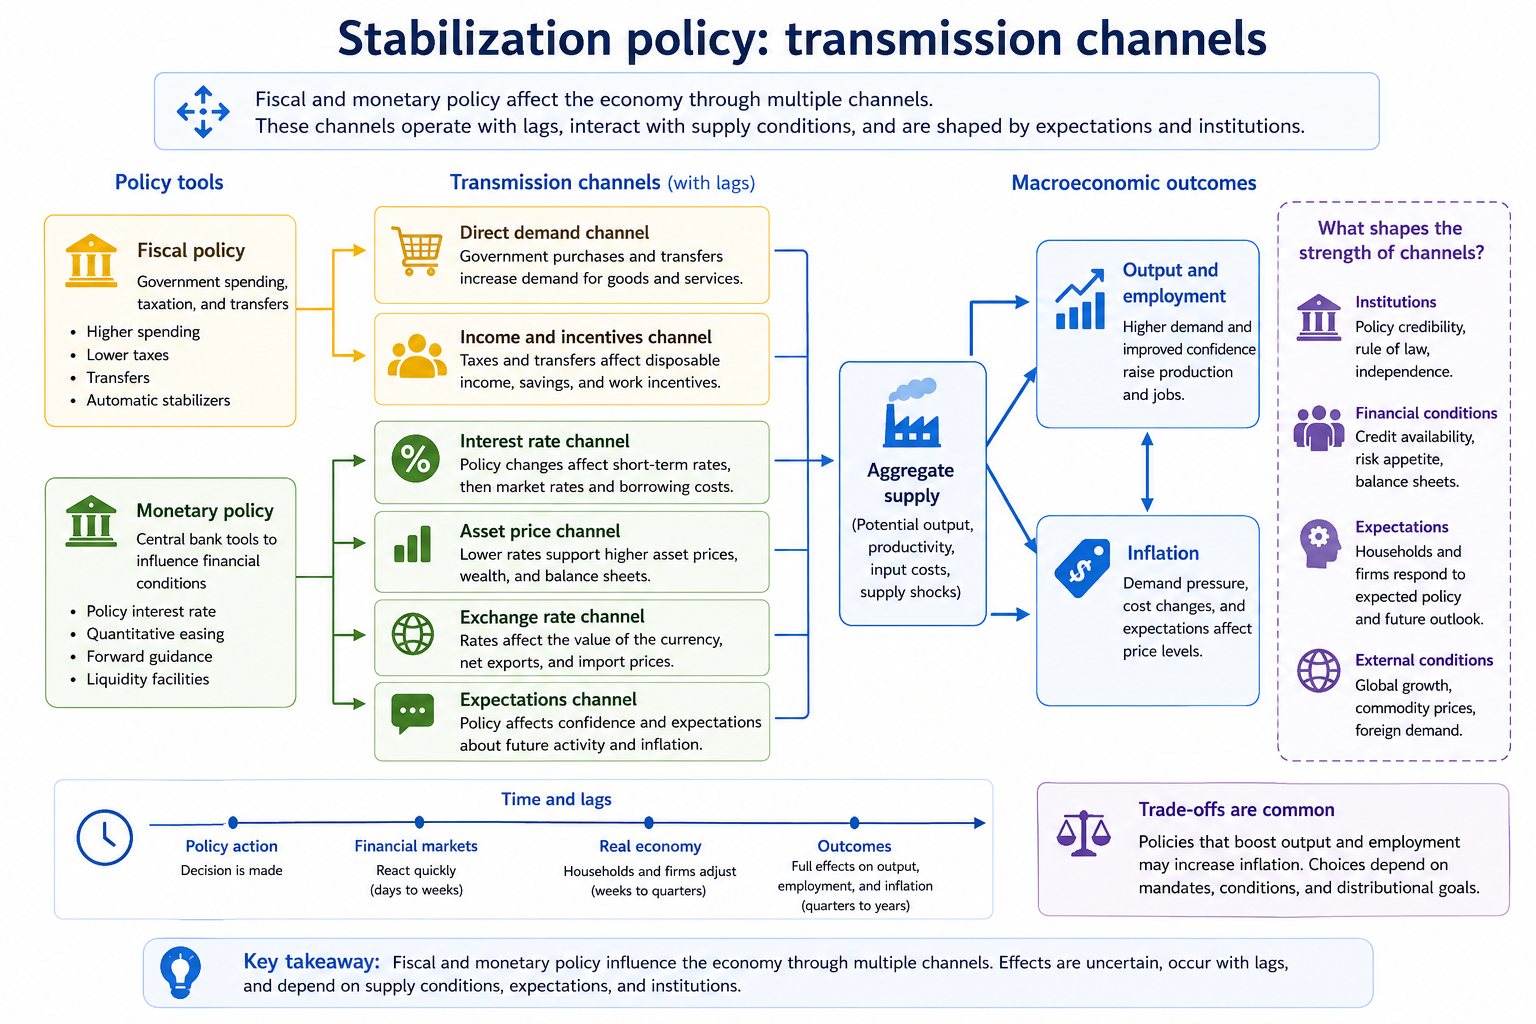
\includegraphics[width=1\linewidth]{images/04_policy_transmission} 

}

\caption{Transmission channels from fiscal and monetary policy to macroeconomic outcomes. Fiscal and monetary policy influence output, employment, and inflation through multiple channels, including interest rates, expectations, income effects, and financial conditions. The strength of these channels depends on institutions, expectations, and economic conditions.}\label{fig:fig-policy-transmission}
\end{figure}

Figure \ref{fig:fig-policy-transmission} illustrates how fiscal and monetary policy affect the economy through several interconnected transmission channels. Fiscal policy influences aggregate demand directly through government spending, taxation, and transfers, while monetary policy affects borrowing conditions, asset prices, exchange rates, and expectations.

The figure also emphasizes that policy effects operate with lags and depend heavily on institutions, credibility, financial conditions, and expectations. The same policy action may therefore produce different outcomes across countries, sectors, or time periods.

\section{Fiscal policy, deficits, and stabilization}\label{fiscal-policy-deficits-and-stabilization}

Fiscal policy refers to government decisions regarding public spending, taxation, and transfers. Governments use fiscal policy to influence economic activity, stabilize business cycles, provide public services, and pursue long-run social and economic objectives.

Government spending affects aggregate demand directly because purchases of goods, services, and infrastructure increase economic activity. Taxation and transfers influence disposable income, consumption, savings, and work incentives.

Fiscal policy may operate automatically or through deliberate intervention. \emph{Automatic stabilizers} are features of the fiscal system that reduce fluctuations without requiring new legislation. Progressive taxation and unemployment insurance are common examples. During recessions, tax revenues often fall while transfer payments increase automatically, partially cushioning declines in household income and demand.

\emph{Discretionary fiscal policy}, in contrast, involves deliberate changes in taxation or spending decisions. Governments may increase infrastructure spending, provide temporary tax reductions, or introduce emergency support programs during economic downturns.

Economists often discuss fiscal policy using the idea of \emph{fiscal multipliers}, which describe how initial changes in government spending or taxation can generate broader changes in economic activity. For example, increased government spending may raise household income, which then increases consumption and generates additional rounds of economic activity.

Fiscal policy also raises questions about deficits and public debt. Budget deficits occur when government spending exceeds revenue during a given period, while public debt reflects the accumulation of past deficits over time.

Debt sustainability depends on several factors, including economic growth, borrowing costs, institutional credibility, and the government's ability to raise revenue. A country with strong institutions and stable growth may sustain higher debt levels more easily than a country facing financial instability or weak revenue capacity.

Importantly, debt sustainability depends not only on the size of debt, but also on the relationship between interest rates and economic growth. When economic growth exceeds borrowing costs, debt burdens may become easier to manage over time.

\section{Monetary policy and financial conditions}\label{monetary-policy-and-financial-conditions}

Monetary policy is typically conducted by central banks, which are often given mandates related to inflation control, employment stabilization, financial stability, or economic growth.

Central banks influence the economy primarily by affecting short-term interest rates and broader financial conditions. When central banks lower policy interest rates, borrowing costs tend to decline, encouraging consumption, investment, and lending. Higher interest rates generally have the opposite effect by discouraging borrowing and slowing demand growth.

Figure \ref{fig:fig-policy-transmission} highlights several important monetary transmission channels. Interest rate changes affect borrowing costs for households and firms, influence asset prices such as housing and equities, alter exchange rates, and shape expectations about future economic conditions.

Expectations are especially important in modern macroeconomics. Households, firms, and financial markets respond not only to current policy, but also to what they believe policymakers will do in the future. Central bank credibility therefore plays an important role in shaping inflation expectations and financial behaviour.

In addition to conventional interest rate policy, central banks may also use \emph{unconventional monetary policy} tools during severe downturns or financial crises. These tools can include quantitative easing, forward guidance, liquidity facilities, and large-scale asset purchases.

Monetary policy also interacts closely with financial stability. Rapid credit growth, asset bubbles, or excessive leverage may create systemic risks even when inflation appears stable. As a result, policymakers sometimes use additional tools such as macroprudential regulation, capital requirements, or lending restrictions to support financial stability.

\section{Transmission lags, uncertainty, and policy trade-offs}\label{transmission-lags-uncertainty-and-policy-trade-offs}

Economic policy operates with significant lags and uncertainty. Financial markets may react quickly to policy announcements, but households and firms often adjust spending, investment, and hiring decisions more gradually. The full effects of policy changes on output, employment, and inflation may take months or even years to emerge.

These lags create major challenges for policymakers because economic conditions may change before the full effects of earlier decisions become visible. Policymakers must therefore make decisions using incomplete information and uncertain forecasts.

Economic policy also involves important trade-offs. Policies designed to reduce inflation may slow economic activity and increase unemployment in the short run. Policies intended to stimulate employment and output may increase inflationary pressures or public debt.

Distributional consequences are also important. Interest rate increases may reduce inflation but increase mortgage costs for borrowers. Fiscal stimulus may support employment while distributing benefits unevenly across sectors or income groups. Tax changes may influence different households in very different ways depending on income, wealth, and consumption patterns.

Policymakers often attempt to achieve a ``soft landing,'' where inflation slows without causing a severe recession or sharp increases in unemployment. Achieving this balance is difficult because economies are shaped by changing expectations, supply shocks, political constraints, and global financial conditions.

The strength of policy transmission channels also differs across institutional and economic contexts. Countries with highly developed financial systems may experience stronger monetary transmission, while countries with weaker institutions or large informal sectors may respond differently to the same policy tools.

\section{Common pitfalls and key takeaways}\label{common-pitfalls-and-key-takeaways-2}

Several common misunderstandings appear repeatedly in discussions of stabilization policy. One is treating policy effects as immediate rather than recognizing the importance of transmission lags. Another is assuming that fiscal and monetary policy work identically across countries or periods.

It is also important not to confuse short-run stabilization policy with long-run structural reform. Policies designed to reduce a recession may differ substantially from policies intended to improve productivity, education, infrastructure, or long-run growth.

Distributional impacts should not be ignored when evaluating stabilization policy. Policies that appear effective in aggregate terms may affect households, industries, and regions very differently.

Overall, fiscal and monetary policy influence the economy through multiple interconnected channels involving demand, expectations, financial conditions, and institutions. Their effectiveness depends not only on the policies themselves, but also on credibility, timing, economic conditions, and distributional context. Good policy evaluation therefore requires considering both effectiveness and equity rather than focusing solely on aggregate outcomes.

\chapter{Ordinary Least Squares (OLS): Simple Linear Regression}\label{ols}

Ordinary Least Squares (OLS) regression is one of the most widely used statistical tools for studying relationships between variables. Researchers use OLS to estimate associations, make predictions, and summarize patterns in data. OLS is popular because it is relatively simple to interpret, computationally efficient, and often provides a useful baseline model before moving to more advanced methods.

In economics, public policy, environmental science, healthcare, and social research, regression models are frequently used to estimate how outcomes change with exposure to different factors. For example, researchers may study how income changes with education, how pollution affects health outcomes, or how policy interventions relate to employment or spending behaviour.

However, regression models must be interpreted carefully. A model may fit the data reasonably well while still producing misleading inference if important assumptions fail. Understanding residuals, diagnostics, assumptions, and model limitations is therefore as important as interpreting coefficients themselves.

This chapter explains what OLS estimates, how coefficients and residuals should be interpreted, why assumptions matter, and how diagnostics help identify potential model problems. It also emphasizes a critical principle in applied statistics: regression alone does not establish causation.

\section{Learning objectives}\label{learning-objectives-4}

By the end of this chapter, you should be able to:

\begin{itemize}
\tightlist
\item
  interpret regression coefficients as conditional associations;
\item
  explain residuals and why OLS minimizes squared errors;
\item
  recognize major OLS assumptions and why violations matter;
\item
  interpret common regression output statistics; and
\item
  identify basic diagnostic patterns and practical responses when assumptions fail.
\end{itemize}

\begin{figure}

{\centering 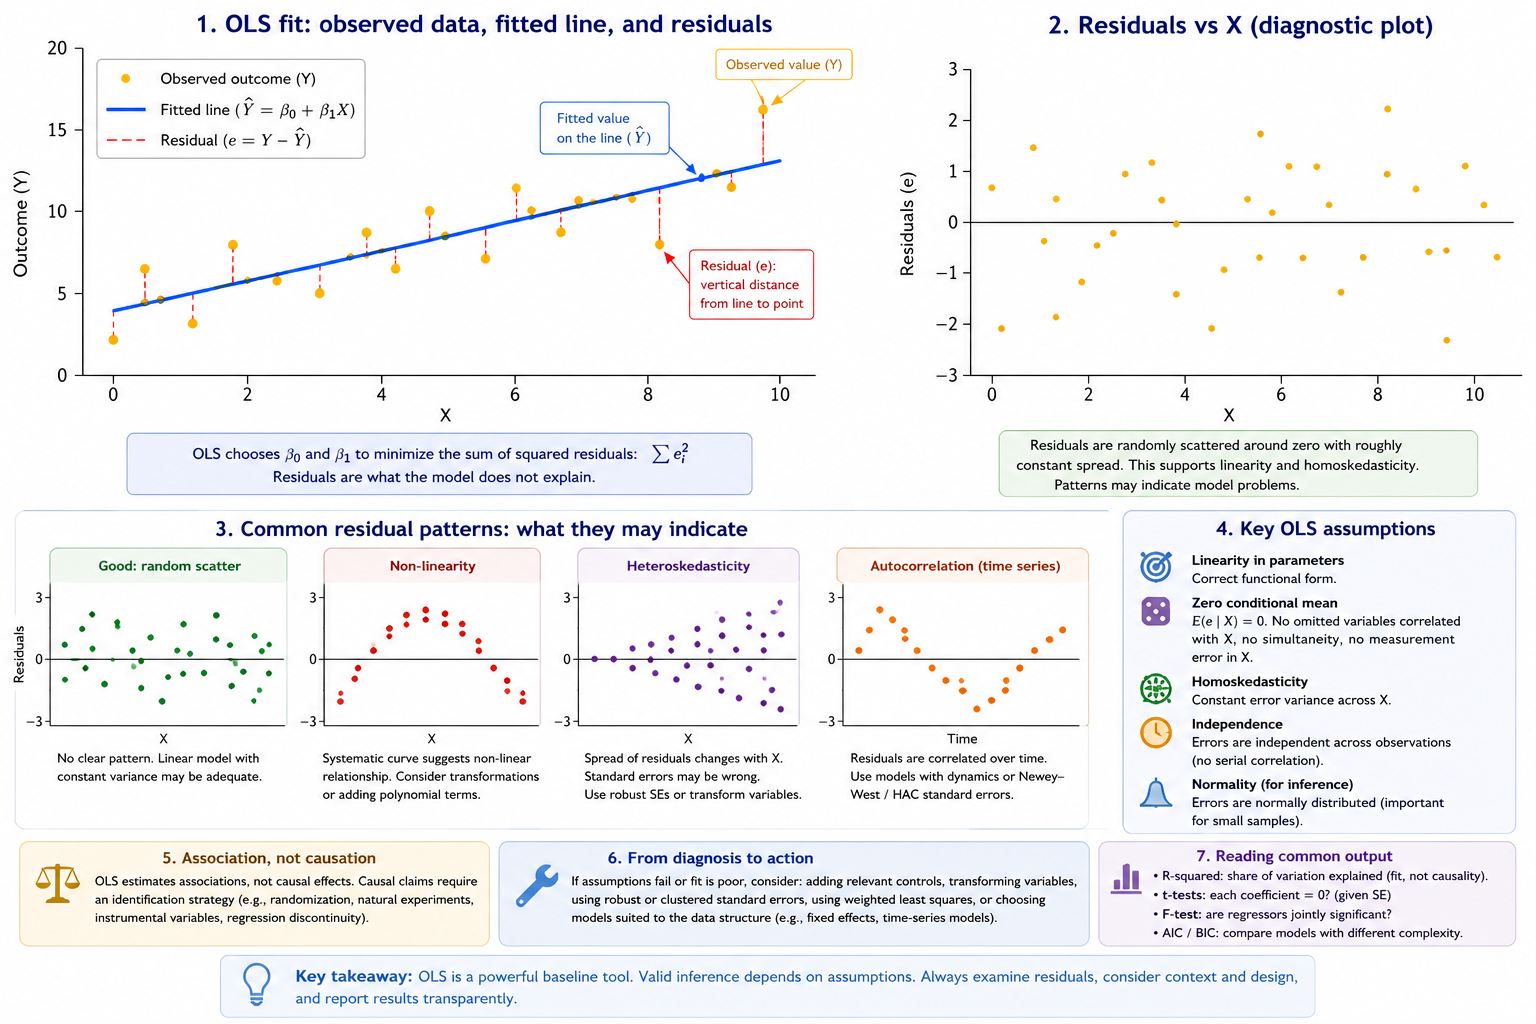
\includegraphics[width=1\linewidth]{images/05_ols_with_residuals} 

}

\caption{OLS fit, residual intuition, and diagnostic patterns. Residuals represent the difference between observed and predicted values. Random residual patterns support the use of a linear model, while systematic patterns may indicate non-linearity, heteroskedasticity, omitted variables, or serial correlation.}\label{fig:fig-ols-resid}
\end{figure}

Figure \ref{fig:fig-ols-resid} illustrates several core ideas behind OLS regression. The upper-left panel shows observed data points together with the fitted regression line. The vertical distance between an observed value and the fitted line is called the \emph{residual}. Residuals represent the portion of the outcome that the model does not explain.

OLS chooses the regression line that minimizes the sum of squared residuals. Squaring residuals ensures that positive and negative errors do not cancel each other out and places greater weight on larger errors.

The residual diagnostic plots in Figure \ref{fig:fig-ols-resid} are equally important. Regression interpretation depends not only on the fitted relationship itself, but also on the remaining structure in the residuals. Random residual scatter around zero generally supports the use of a linear model with approximately constant variance. Systematic residual patterns, however, may indicate problems such as non-linearity, heteroskedasticity, omitted variables, or serial correlation.

\section{What OLS estimates}\label{what-ols-estimates}

In a simple linear regression, the estimated coefficient summarizes the average change in the outcome associated with a one-unit change in the predictor variable.

In multiple regression models, coefficients are interpreted as \emph{conditional associations}. This means the coefficient describes how the outcome changes with one variable while holding the other included variables constant.

For example, in a regression of wages on education and experience, the education coefficient estimates the association between education and wages conditional on the level of experience included in the model.

It is important to recognize that regression estimates associations, not necessarily causal effects. Two variables may move together because one causes the other, because both are influenced by a third factor, or because of reverse causality.

For example, ice cream sales and drowning incidents may both increase during summer months. A regression may detect a positive association even though ice cream consumption does not cause drowning. Temperature acts as a confounding factor influencing both variables simultaneously.

Because of this, causal interpretation requires careful research design rather than regression alone.

\section{Residuals, assumptions, and inference}\label{residuals-assumptions-and-inference}

Residuals play a central role in regression analysis because they help evaluate whether model assumptions appear reasonable.

One important assumption is \emph{linearity}, meaning the relationship between predictors and the outcome is reasonably approximated by a linear function. Curved residual patterns may suggest that transformations or non-linear terms are needed.

Another important assumption is \emph{homoskedasticity}, which means the variance of residuals remains relatively constant across levels of the predictor variables. When residual spread changes systematically, a problem called \emph{heteroskedasticity} occurs. Heteroskedasticity does not necessarily bias coefficient estimates, but it can produce incorrect standard errors and misleading statistical inference.

Figure \ref{fig:fig-ols-resid} includes an example of heteroskedasticity where residual variance changes across the range of observations.

A particularly important assumption for causal interpretation is the \emph{zero conditional mean assumption}. Informally, this means that omitted factors affecting the outcome should not be systematically correlated with included predictors. Violations often arise because of omitted variables, simultaneity, measurement error, or selection bias.

For example, if ability influences both education and income but is omitted from the regression, the estimated education coefficient may partially capture the effect of ability rather than education alone.

Independence of errors is another important assumption. In cross-sectional data, observations are often assumed to be independent. In time-series data, however, residuals are frequently correlated over time. This problem, known as \emph{serial correlation} or \emph{autocorrelation}, can distort inference if ignored.

The residual examples in Figure \ref{fig:fig-ols-resid} show how systematic patterns may reveal these types of problems.

\section{Reading regression output}\label{reading-regression-output}

Regression software typically reports several statistics that summarize model fit and uncertainty.

One commonly reported statistic is \emph{R-squared}, which measures the proportion of variation in the outcome explained by the model. A higher R-squared indicates better statistical fit, but it does not guarantee that the model is theoretically meaningful or causally valid.

A model may fit the observed data well while still omitting important variables or using an incorrect functional form.

Regression output also reports \emph{standard errors}, \emph{t-tests}, and \emph{p-values}, which help evaluate statistical uncertainty around coefficient estimates. A t-test evaluates whether a coefficient differs significantly from zero given estimated uncertainty.

The \emph{F-test} evaluates whether groups of variables are jointly important in explaining the outcome.

When comparing models, researchers may also use criteria such as AIC and BIC, which balance model fit against model complexity. These measures discourage excessive overfitting by penalizing models that include too many predictors relative to the information gained.

\section{Diagnostics and practical responses}\label{diagnostics-and-practical-responses}

Diagnostics help determine whether a regression model appears appropriate for the data structure and research question.

Figure \ref{fig:fig-ols-resid} illustrates several common residual patterns. Random scatter around zero generally supports the use of a linear specification with approximately constant variance. Curved residual patterns may indicate non-linearity, funnel-shaped patterns may suggest heteroskedasticity, and systematic time patterns may indicate autocorrelation.

When assumptions appear violated, researchers often modify the model or adjust inference methods. Common responses include:

\begin{itemize}
\tightlist
\item
  adding relevant control variables;
\item
  transforming variables using logarithms or polynomial terms;
\item
  using robust standard errors;
\item
  using clustered or heteroskedasticity-consistent standard errors;
\item
  or choosing models better suited to the data structure, such as time-series or panel-data methods.
\end{itemize}

Robust standard errors are especially common in applied work because real-world data frequently violate constant variance assumptions.

The example below shows a simplified OLS workflow using robust standard errors.

\begin{Shaded}
\begin{Highlighting}[]
\CommentTok{\# Example data (simulated)}
\FunctionTok{set.seed}\NormalTok{(}\DecValTok{1}\NormalTok{)}

\NormalTok{df }\OtherTok{\textless{}{-}} \FunctionTok{data.frame}\NormalTok{(}
  \AttributeTok{outcome =} \FunctionTok{rnorm}\NormalTok{(}\DecValTok{100}\NormalTok{),}
  \AttributeTok{exposure =} \FunctionTok{rbinom}\NormalTok{(}\DecValTok{100}\NormalTok{, }\DecValTok{1}\NormalTok{, }\FloatTok{0.5}\NormalTok{),}
  \AttributeTok{age =} \FunctionTok{sample}\NormalTok{(}\DecValTok{18}\SpecialCharTok{:}\DecValTok{90}\NormalTok{, }\DecValTok{100}\NormalTok{, }\ConstantTok{TRUE}\NormalTok{),}
  \AttributeTok{sex =} \FunctionTok{sample}\NormalTok{(}\FunctionTok{c}\NormalTok{(}\StringTok{"F"}\NormalTok{,}\StringTok{"M"}\NormalTok{), }\DecValTok{100}\NormalTok{, }\ConstantTok{TRUE}\NormalTok{)}
\NormalTok{)}

\CommentTok{\# Baseline OLS model}
\NormalTok{fit }\OtherTok{\textless{}{-}} \FunctionTok{lm}\NormalTok{(outcome }\SpecialCharTok{\textasciitilde{}}\NormalTok{ exposure }\SpecialCharTok{+}\NormalTok{ age }\SpecialCharTok{+}\NormalTok{ sex, }\AttributeTok{data =}\NormalTok{ df)}

\CommentTok{\# Standard regression output}
\FunctionTok{summary}\NormalTok{(fit)}

\CommentTok{\# Robust standard errors}
\FunctionTok{library}\NormalTok{(sandwich)}
\FunctionTok{library}\NormalTok{(lmtest)}

\FunctionTok{coeftest}\NormalTok{(fit, }\AttributeTok{vcov. =} \FunctionTok{vcovHC}\NormalTok{(fit, }\AttributeTok{type =} \StringTok{"HC1"}\NormalTok{))}
\end{Highlighting}
\end{Shaded}

This workflow reflects a common applied approach where OLS provides a baseline model and robust standard errors help account for possible heteroskedasticity.

\section{Common pitfalls and key takeaways}\label{common-pitfalls-and-key-takeaways-3}

Several common misunderstandings appear frequently in regression analysis. One is interpreting regression coefficients causally without an appropriate identification strategy or research design. Another is treating R-squared as a measure of truth rather than simply a measure of fit.

Researchers may also ignore heteroskedasticity or serial correlation, leading to incorrect inference even when coefficient estimates themselves appear reasonable. Overfitting is another common problem, particularly when many predictors are included without theoretical justification.

Overall, OLS regression is a powerful and widely used baseline method for analyzing relationships between variables. However, valid inference depends on assumptions, diagnostics, and research design rather than on regression output alone. Residual analysis and model diagnostics should therefore be treated as central parts of statistical interpretation rather than optional afterthoughts.

Most importantly, causal claims require careful design, theory, and identification strategies---not regression alone.

\chapter{Multivariate Modeling}\label{multivariate}

Applied questions often involve multiple predictors and sometimes multiple outcomes. Multivariate modeling generalizes regression thinking and raises important inference issues such as multiple testing and joint interpretation.

Roadmap

We clarify terminology, then discuss interpretation when many predictors or outcomes are present. We close with practical guidance on specification and communication.

Learning objectives

\begin{itemize}
\tightlist
\item
  Distinguish multiple regression from multivariate multiple regression.
\item
  Explain why joint inference matters when outcomes are multiple.
\item
  Describe the role of controls and interaction terms.
\item
  Recognize risks of multiple comparisons and overfitting.
\item
  Communicate multivariate results clearly for policy audiences.
\end{itemize}

\begin{figure}

{\centering 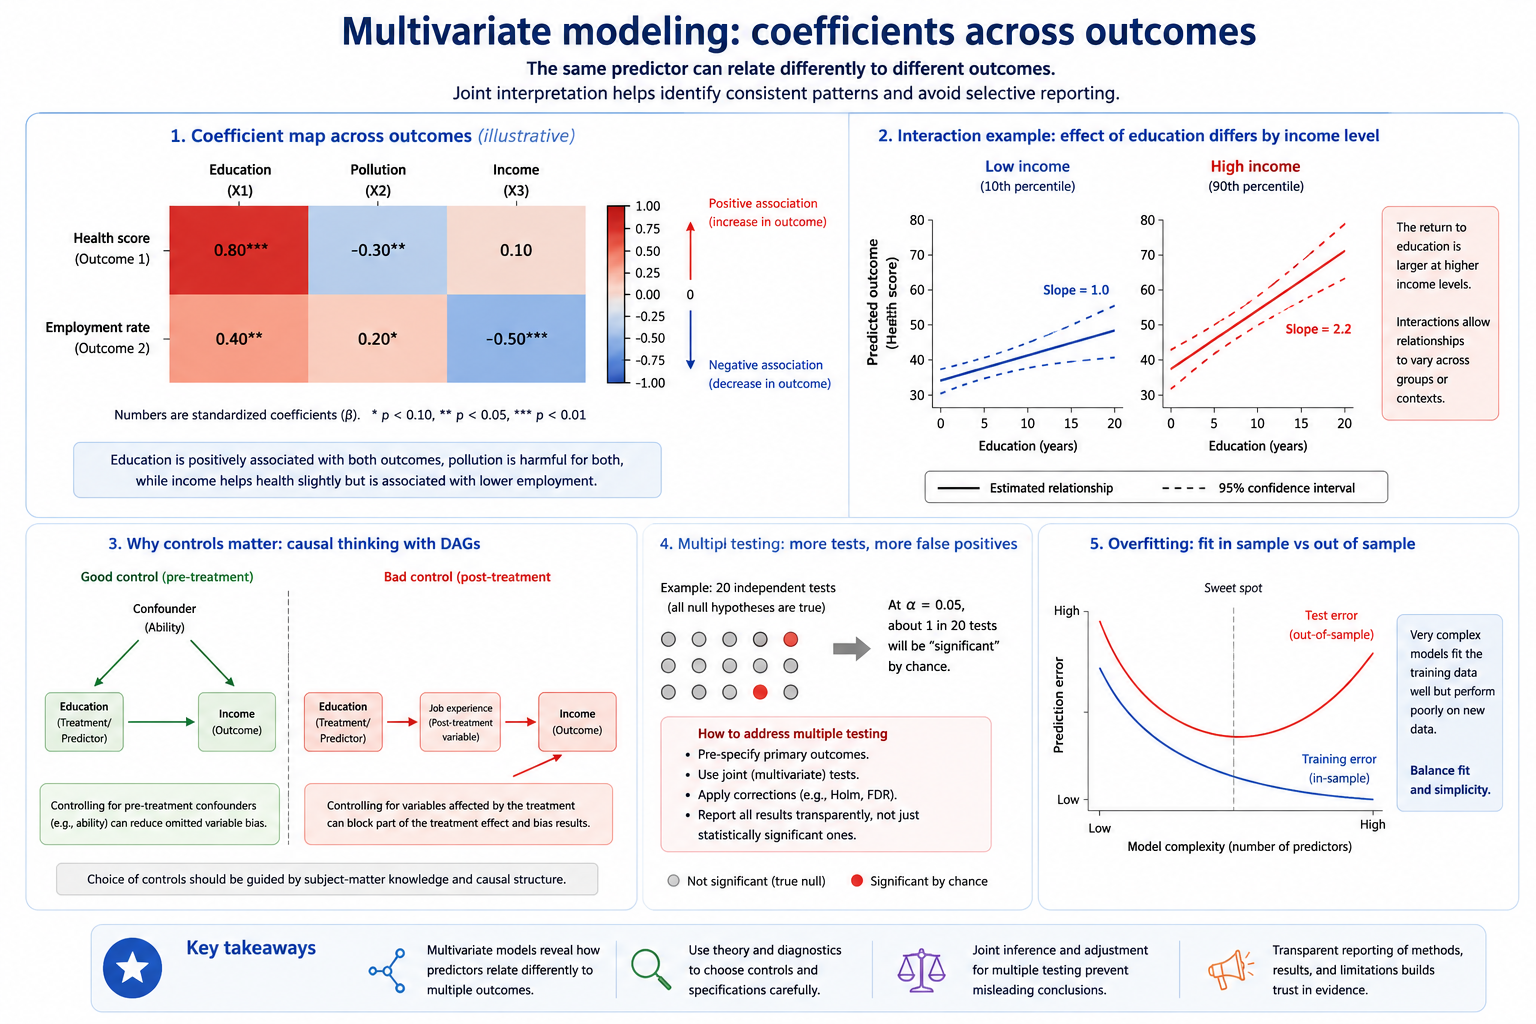
\includegraphics[width=0.95\linewidth]{images/06_multivariate_coefficients} 

}

\caption{Illustrative coefficient map across outcomes. The same predictor can relate differently to different outcomes, motivating joint interpretation and careful reporting.}\label{fig:fig-multi-coef}
\end{figure}

Figure \ref{fig:fig-multi-coef} illustrates why multivariate work requires careful interpretation. Differences across outcomes can reflect mechanisms, measurement, or specification choices.

\section{Multiple regression}\label{multiple-regression}

Multiple regression uses multiple predictors to explain one outcome. Controls can reduce confounding when they capture relevant omitted factors.

However, controls can also introduce bias if they are affected by the treatment (post-treatment variables). In evaluation contexts, the causal graph matters.

\section{Multivariate multiple regression}\label{multivariate-multiple-regression}

Multivariate multiple regression models multiple outcomes using the same predictors. It is useful when outcomes are related and when you want a coherent story across measures.

\section{Inference with many outcomes}\label{inference-with-many-outcomes}

Testing many outcomes increases false positives. Strategies include focusing on primary outcomes, using joint tests, and applying corrections.

\section{Practical reporting}\label{practical-reporting}

Good reporting states:

\begin{itemize}
\tightlist
\item
  which outcomes were primary
\item
  how multiple testing was handled
\item
  whether results are robust across specifications
\item
  how effects translate into meaningful units
\end{itemize}

Common pitfalls

\begin{itemize}
\tightlist
\item
  Treating a long list of significant results as strong evidence without correction.
\item
  Using controls mechanically without considering causal structure.
\item
  Reporting only significant outcomes and omitting the full set.
\end{itemize}

Key takeaways

\begin{itemize}
\tightlist
\item
  Multivariate models can strengthen evidence when designed carefully.
\item
  Joint inference and transparent reporting prevent misleading conclusions.
\end{itemize}

\chapter{Time Series Forecasting Theory (AR, MA, ARMA, ARIMA)}\label{time-series}

Time series data record observations sequentially through time. Unlike cross-sectional data, where observations are often treated as independent, time series observations are usually connected to past values and past shocks. Forecasting therefore requires understanding how patterns evolve over time and whether those patterns are stable enough to support prediction.

Economic, environmental, financial, and public health data frequently exhibit trends, cycles, persistence, and seasonal behaviour. Monthly unemployment rates, annual GDP, river discharge, inflation, electricity demand, and disease incidence are all examples of time series data.

Forecasting models attempt to capture systematic structure while avoiding overfitting random fluctuations. Good forecasting therefore depends not only on model selection, but also on understanding the underlying behaviour of the series itself.

This chapter introduces the main components of time series data, explains the idea of stationarity, develops intuition for autoregressive and moving-average models, and concludes with the logic of ARIMA forecasting and practical diagnostic workflows.

\section{Learning objectives}\label{learning-objectives-5}

By the end of this chapter, you should be able to:

\begin{itemize}
\tightlist
\item
  identify trend, seasonality, cycles, and noise in a time series;
\item
  explain stationarity and why differencing may be necessary;
\item
  describe the intuition behind AR and MA processes;
\item
  interpret ARIMA notation and seasonal extensions; and
\item
  outline a practical forecasting workflow using diagnostics and residual checks.
\end{itemize}

\begin{figure}

{\centering 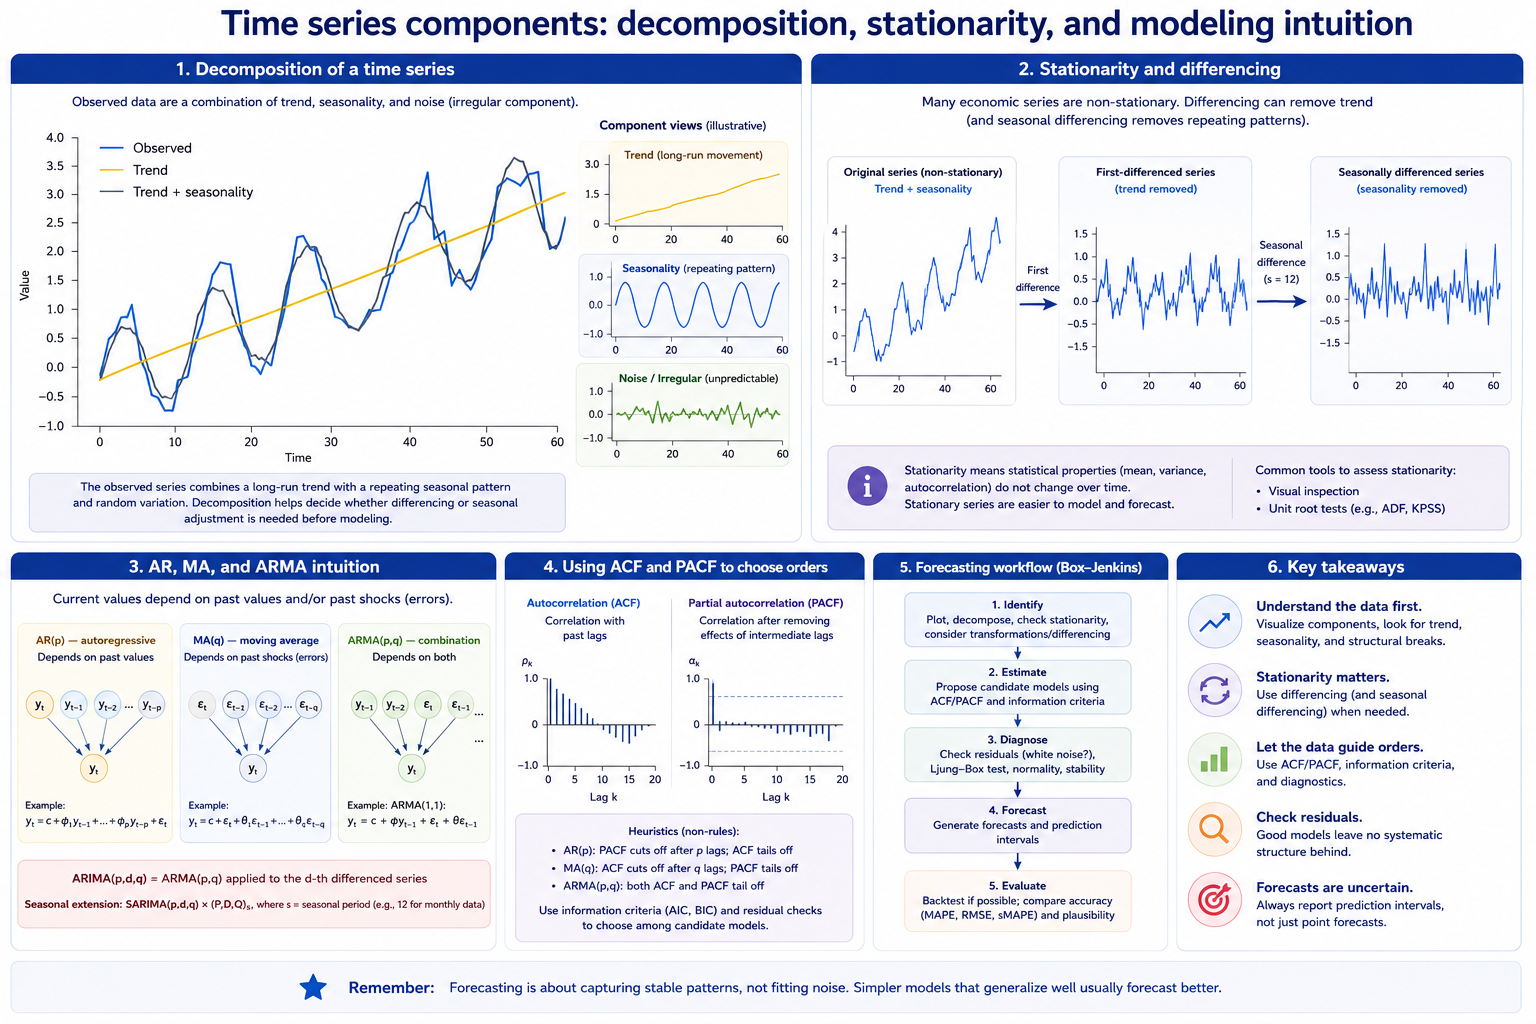
\includegraphics[width=1\linewidth]{images/07_time_series_components} 

}

\caption{Illustrative decomposition of a time series into trend and seasonal components. The observed series combines long-run growth, repeating seasonal fluctuations, and random variation. Decomposition helps identify structure and supports decisions about differencing, seasonal adjustment, and model selection.}\label{fig:fig-ts-components}
\end{figure}

Figure \ref{fig:fig-ts-components} illustrates one of the central ideas in forecasting: observed time series often contain multiple overlapping components rather than pure randomness. The blue line represents the observed data, while the trend and seasonal components help explain systematic movement over time.

The upward-sloping trend in Figure \ref{fig:fig-ts-components} reflects long-run growth, while the repeating oscillations represent seasonality. Forecasting models attempt to capture these predictable structures without fitting random noise too aggressively.

\section{Components of time series data}\label{components-of-time-series-data}

Time series data are often described as combinations of several components.

A \emph{trend} represents long-run movement in the series. Economic growth, population increase, technological progress, and climate warming are examples of trend behaviour.

\emph{Seasonality} refers to patterns that repeat at regular intervals such as months, quarters, or days of the week. Retail sales often increase during holidays, electricity demand may rise during winter or summer months, and tourism activity frequently follows seasonal cycles.

\emph{Cycles} are longer-term fluctuations that do not necessarily repeat at fixed intervals. Business cycles are a common example. Unlike seasonality, cyclical behaviour may vary substantially in duration and magnitude.

The remaining variation is often described as \emph{noise} or \emph{irregular variation}. This component represents unpredictable shocks and random fluctuations that forecasting models may not explain well.

Visualization is one of the most important first steps in time-series analysis. Plotting the series often reveals trends, structural breaks, changing variance, or seasonality before formal modeling begins.

A series that resembles pure white noise contains little predictable structure and is difficult to forecast beyond its historical average.

\section{Stationarity and differencing}\label{stationarity-and-differencing}

Many time-series methods assume that the statistical properties of the series remain relatively stable over time. This property is known as \emph{stationarity}.

Informally, a stationary series has a stable mean, stable variance, and stable autocorrelation structure through time. In contrast, many real-world economic and environmental series exhibit trends, changing variance, or evolving dependence structures.

Non-stationary data can create misleading statistical relationships and unstable forecasts. For this reason, transforming the series is often necessary before fitting forecasting models.

One common transformation is \emph{differencing}, which removes long-run trend behaviour by analyzing changes between consecutive observations rather than the original levels themselves.

For example, instead of modeling GDP directly, analysts may model changes in GDP from one period to the next.

Seasonal differencing can also remove repeating seasonal patterns by subtracting observations from previous seasonal periods.

Figure \ref{fig:fig-ts-components} illustrates why differencing may be useful. The upward trend and recurring seasonal fluctuations suggest that the original series may not satisfy stationarity assumptions in its raw form.

The following template illustrates a simple workflow for visually checking stationarity and applying differencing.

\begin{Shaded}
\begin{Highlighting}[]
\CommentTok{\# Example time series object}
\NormalTok{y\_ts }\OtherTok{\textless{}{-}} \FunctionTok{ts}\NormalTok{(y, }\AttributeTok{frequency =} \DecValTok{12}\NormalTok{)}

\CommentTok{\# Plot original series}
\FunctionTok{plot}\NormalTok{(y\_ts, }\AttributeTok{main =} \StringTok{"Time series (raw)"}\NormalTok{)}

\CommentTok{\# First differencing}
\NormalTok{dy }\OtherTok{\textless{}{-}} \FunctionTok{diff}\NormalTok{(y\_ts)}

\CommentTok{\# Plot differenced series}
\FunctionTok{plot}\NormalTok{(dy, }\AttributeTok{main =} \StringTok{"First difference"}\NormalTok{)}

\CommentTok{\# Optional formal stationarity test}
\FunctionTok{library}\NormalTok{(tseries)}

\FunctionTok{adf.test}\NormalTok{(y\_ts)}
\FunctionTok{adf.test}\NormalTok{(}\FunctionTok{na.omit}\NormalTok{(dy))}
\end{Highlighting}
\end{Shaded}

Visual inspection remains important even when formal tests are used. Statistical tests may have limited power in small samples or produce conflicting conclusions when structural breaks or seasonal patterns are present.

\section{AR, MA, and ARIMA intuition}\label{ar-ma-and-arima-intuition}

Many forecasting models are built around the idea that current values depend on past values and past shocks.

An \emph{autoregressive} (AR) model assumes that the current value depends on previous observations in the series itself. For example, unemployment this month may depend partly on unemployment last month.

A \emph{moving-average} (MA) model instead assumes that current values depend on past shocks or forecast errors. In this framework, temporary disturbances can continue to influence the series for several periods.

An \emph{ARMA} model combines both autoregressive and moving-average behaviour. These models are useful when the series is already stationary.

Many real-world series, however, are non-stationary. \emph{ARIMA} models extend ARMA models by adding differencing to remove trend behaviour before modeling the remaining structure.

The notation ARIMA\((p,d,q)\) summarizes the model structure:

\begin{itemize}
\tightlist
\item
  \(p\) represents the autoregressive order;
\item
  \(d\) represents the degree of differencing; and
\item
  \(q\) represents the moving-average order.
\end{itemize}

Seasonal extensions such as SARIMA models add additional seasonal autoregressive, differencing, and moving-average components.

Autocorrelation diagnostics help guide model selection. The \emph{autocorrelation function} (ACF) measures correlation between observations separated by different time lags, while the \emph{partial autocorrelation function} (PACF) measures correlation after controlling for intermediate lags.

Analysts often examine ACF and PACF plots together with information criteria such as AIC and BIC to propose candidate model orders.

\section{Forecasting workflow and diagnostics}\label{forecasting-workflow-and-diagnostics}

Time-series forecasting is typically an iterative process rather than a single modeling step.

A common workflow begins with visualization and decomposition to identify trend, seasonality, structural breaks, and unusual observations. The series may then be transformed or differenced to improve stationarity.

After selecting candidate models, analysts estimate parameters and evaluate residual diagnostics. Good forecasting models should leave residuals that resemble white noise, meaning that little systematic structure remains unexplained.

Residual autocorrelation, changing variance, or remaining seasonality may indicate that the model is incomplete or misspecified.

Forecast evaluation should also consider plausibility and uncertainty rather than focusing only on point forecasts. Forecast intervals are often more informative than single predicted values because uncertainty generally increases further into the future.

Overfitting is another important concern. Highly complex models may fit historical data extremely well while performing poorly on future observations. Forecasting therefore requires balancing flexibility with generalization.

Several common pitfalls appear repeatedly in applied forecasting work. Analysts may fit ARIMA models to clearly non-stationary data without differencing, ignore visible seasonality, or select excessively high model orders that fit noise rather than meaningful structure.

It is also important not to treat forecasts as certainty. Forecasts are probabilistic statements shaped by assumptions, historical patterns, and model limitations.

Overall, time-series forecasting combines statistical modeling with careful diagnostic reasoning. Trend, seasonality, persistence, and shocks all shape how time series evolve over time. Effective forecasting therefore depends not only on choosing a model, but also on understanding the structure and stability of the underlying process.

\chapter{Causality, Identification, and Policy Evaluation}\label{causality}

Policymakers and researchers are often interested in causal questions rather than simple associations. Instead of asking whether two variables move together, policy evaluation typically asks whether a policy, program, intervention, or exposure actually caused an outcome to change.

Examples include questions such as:
- Did a training program increase employment?
- Did a carbon tax reduce emissions?
- Did a healthcare intervention improve patient outcomes?
- Did new policing policies reduce crime?

Answering these questions requires more than statistical correlation. The central challenge in causal inference is determining what would have happened in the absence of the intervention. This unobserved alternative is called the \emph{counterfactual}.

Because the same individual, region, or organization cannot simultaneously experience both treatment and non-treatment at the same time, causal inference requires strategies that approximate the missing counterfactual as credibly as possible.

This chapter introduces the logic of counterfactual reasoning, explains major threats to causal interpretation, and outlines common identification strategies used in applied policy evaluation.

\section{Learning objectives}\label{learning-objectives-6}

By the end of this chapter, you should be able to:

\begin{itemize}
\tightlist
\item
  explain why counterfactual reasoning is central to causal inference;
\item
  identify major threats to causal interpretation;
\item
  describe common identification strategies and their assumptions; and
\item
  evaluate the credibility and robustness of causal evidence.
\end{itemize}

\begin{figure}

{\centering 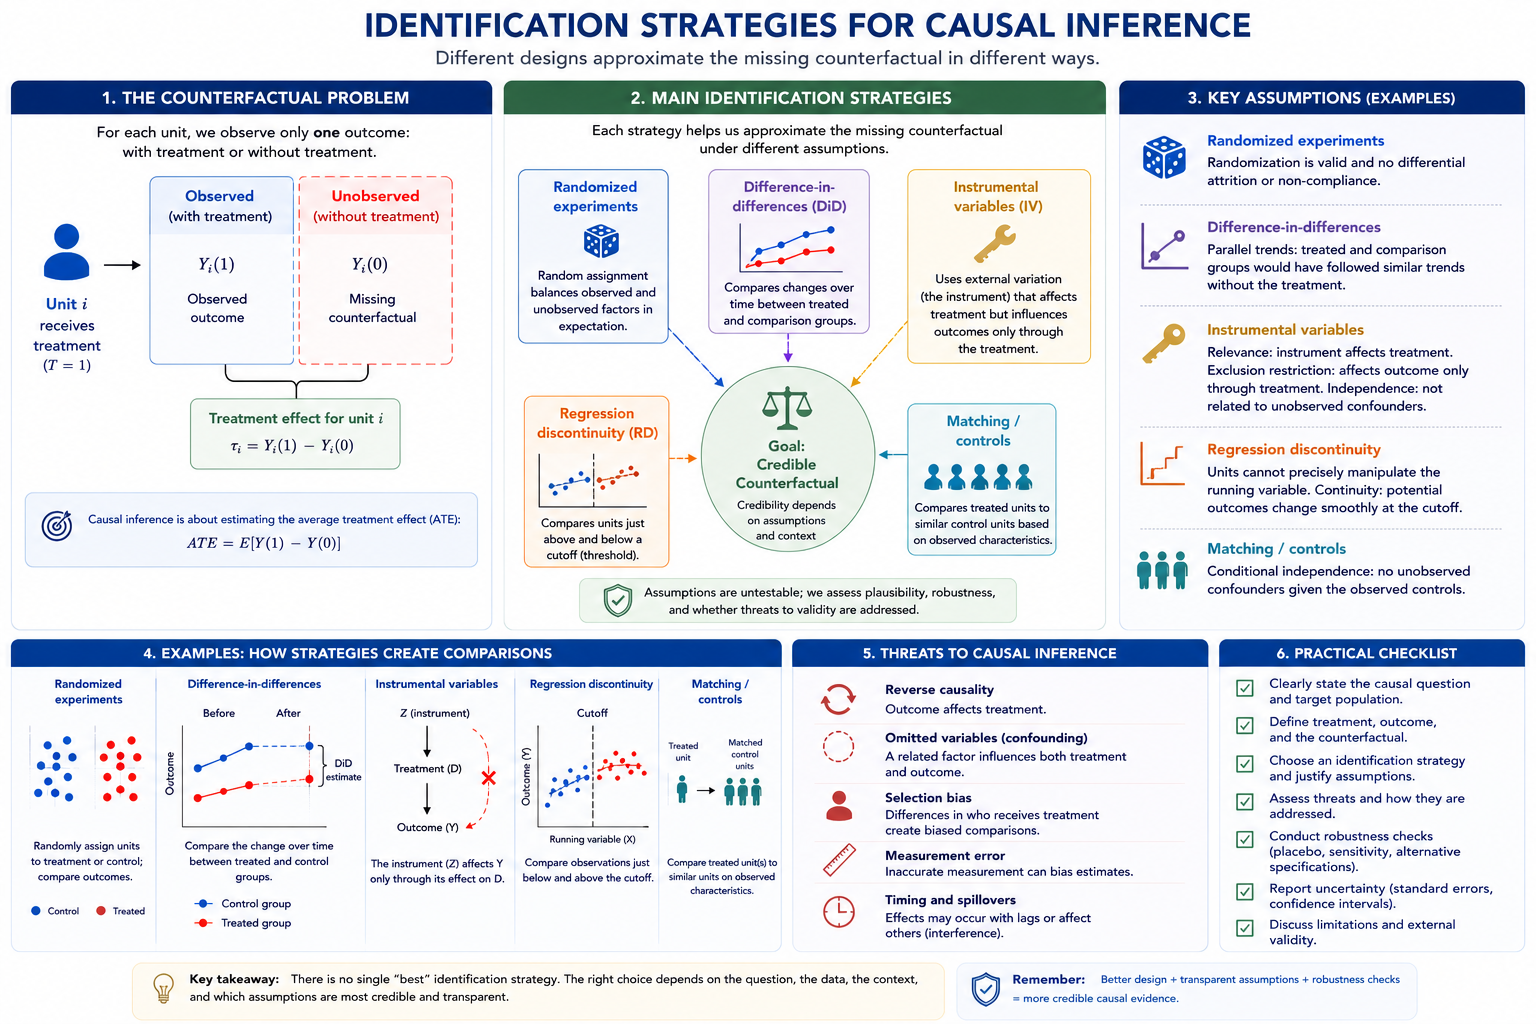
\includegraphics[width=1\linewidth]{images/08_identification_strategies} 

}

\caption{Identification strategies for causal inference. Different research designs approximate the missing counterfactual under different assumptions. Credible causal inference depends not only on statistical models, but also on research design, assumptions, and robustness checks.}\label{fig:fig-identification}
\end{figure}

Figure \ref{fig:fig-identification} summarizes the central problem of causal inference and several common strategies used to address it. The left panel illustrates the \emph{counterfactual problem}: for each unit, we observe either the treated outcome or the untreated outcome, but never both simultaneously.

The remaining panels show how different identification strategies attempt to approximate the missing counterfactual using different forms of comparison. Some approaches rely on random assignment, while others exploit thresholds, timing differences, external variation, or carefully selected comparison groups.

Importantly, Figure \ref{fig:fig-identification} also highlights that all identification strategies depend on assumptions. Credibility therefore depends not only on statistical estimation, but also on whether the assumptions are plausible in the policy context being studied.

\section{Correlation, causation, and the counterfactual problem}\label{correlation-causation-and-the-counterfactual-problem}

Correlation alone does not establish causation. Two variables may move together because one causes the other, because causality operates in the reverse direction, or because both variables are influenced by a third factor.

For example, regions with more hospitals may also have higher mortality rates, not because hospitals increase mortality, but because hospitals are often concentrated in areas with sicker populations. Similarly, education and income are positively associated, but part of this relationship may reflect factors such as family background, ability, or social networks.

The key challenge in causal inference is that we never directly observe the same unit both with and without treatment at the same moment in time. The unobserved outcome without treatment is the missing counterfactual.

Causal inference therefore requires constructing a comparison that approximates what would have happened in the absence of treatment. Different identification strategies attempt to create this comparison in different ways.

Figure \ref{fig:fig-identification} places the counterfactual problem at the center because all causal designs ultimately attempt to approximate this missing comparison.

\section{Threats to causal inference}\label{threats-to-causal-inference}

Several common problems can distort causal interpretation.

One important threat is \emph{reverse causality}, where the outcome itself influences treatment. For example, poor health may reduce income, but low income may also worsen health outcomes.

Another major issue is \emph{omitted variable bias} or \emph{confounding}. Confounding occurs when a third factor affects both treatment assignment and outcomes. If important confounding variables are omitted from the analysis, estimated effects may become biased.

\emph{Selection bias} is also common in policy evaluation. Individuals who receive treatment may differ systematically from those who do not. For example, motivated individuals may be more likely to participate in training programs, making simple comparisons misleading.

Measurement error can further distort estimates if variables are measured inaccurately or inconsistently across groups or time periods.

These threats often occur simultaneously in real-world policy settings, which is why research design is central to credible causal analysis.

\section{Common identification strategies}\label{common-identification-strategies}

Different identification strategies attempt to create credible comparisons under different assumptions.

\subsection{Randomized experiments}\label{randomized-experiments}

Randomized experiments assign treatment randomly across units. Randomization helps balance both observed and unobserved characteristics between treated and control groups, making the groups comparable on average.

Because treatment assignment is independent of participant characteristics, randomized experiments are often considered the strongest design for internal validity. However, experiments may still face challenges such as attrition, non-compliance, ethical constraints, or limited external validity.

Figure \ref{fig:fig-identification} illustrates how randomized assignment attempts to create a valid counterfactual through balanced comparison groups.

\subsection{Difference-in-differences}\label{difference-in-differences}

Difference-in-differences (DiD) compares changes over time between treated and comparison groups. Instead of comparing levels directly, DiD estimates whether outcomes changed differently after treatment relative to a comparison group.

The key assumption is the \emph{parallel trends assumption}, which states that treated and comparison groups would have followed similar trends in the absence of treatment.

Difference-in-differences designs are widely used in policy evaluation because many real-world policies are implemented at different times or across different jurisdictions.

\subsection{Instrumental variables}\label{instrumental-variables}

Instrumental variable (IV) methods use external variation that affects treatment assignment but influences outcomes only through treatment itself.

A valid instrument must satisfy two key conditions:
- it must affect treatment assignment (\emph{relevance}); and
- it must not directly affect the outcome except through treatment (\emph{exclusion restriction}).

Instrumental variables are especially useful when treatment selection is endogenous or affected by unobserved factors.

Figure \ref{fig:fig-identification} emphasizes that IV methods rely heavily on strong assumptions regarding the instrument's validity.

\subsection{Regression discontinuity}\label{regression-discontinuity}

Regression discontinuity (RD) designs exploit thresholds or cutoffs that determine treatment assignment. Units just above and below the threshold are assumed to be comparable except for treatment exposure.

For example, scholarship eligibility based on test scores may create a discontinuity where students near the cutoff are very similar but receive different treatment status.

RD designs often produce highly credible local causal estimates when manipulation around the threshold is limited.

\subsection{Matching and controls}\label{matching-and-controls}

Matching methods and regression controls attempt to compare treated units with observationally similar control units.

These methods can improve comparability when rich covariate information is available. However, matching approaches can only account for observed characteristics. Unobserved confounding may still bias results.

Controls should also not be added mechanically. Variables affected by the treatment itself may introduce \emph{post-treatment bias} and distort causal interpretation.

\section{Robustness, transparency, and policy evaluation}\label{robustness-transparency-and-policy-evaluation}

Credible policy evaluation requires more than estimating a statistically significant coefficient. Researchers must clearly define the causal question, justify assumptions, explain the counterfactual, and evaluate robustness.

Figure \ref{fig:fig-identification} includes a practical evaluation checklist emphasizing transparency, robustness checks, uncertainty reporting, and discussion of limitations.

Robustness checks may include:
- alternative model specifications;
- placebo tests;
- sensitivity analysis;
- alternative control groups;
- or different variable definitions.

Researchers should also discuss implementation details, spillovers, timing issues, and institutional context because these factors may affect whether identification assumptions remain credible.

Importantly, statistical significance alone is not proof of causality. A statistically significant result may still be biased if the identification strategy is weak or assumptions are implausible.

Similarly, causal evidence should always be interpreted together with uncertainty, effect magnitude, external validity, and policy relevance.

\section{Common pitfalls and key takeaways}\label{common-pitfalls-and-key-takeaways-4}

Several common mistakes appear repeatedly in applied policy analysis. One is treating correlation as evidence of causation without addressing confounding or selection bias. Another is relying heavily on statistical models while giving insufficient attention to research design and assumptions.

Researchers may also use controls mechanically without considering causal pathways, or selectively report significant findings while omitting robustness checks and non-significant results.

Overall, causal inference depends fundamentally on design rather than statistical modeling alone. A credible counterfactual, transparent assumptions, and careful robustness analysis are central to trustworthy policy evaluation.

Different identification strategies approximate the counterfactual in different ways, and no single method is universally best. The appropriate strategy depends on the policy question, available variation, institutional context, and the plausibility of the required assumptions.

\chapter{Interrupted Time Series Analysis (ITSA): Concepts}\label{itsa}

Many important policies and interventions cannot be evaluated using randomized experiments. Governments rarely randomize tax changes, healthcare reforms, environmental regulations, or public safety interventions across populations. In these situations, researchers often rely on observational designs that attempt to estimate what would have happened in the absence of the intervention.

Interrupted time series analysis (ITSA) is one of the strongest quasi-experimental approaches available when interventions occur at a clearly identifiable point in time and repeated observations are available before and after implementation.

The central idea behind ITSA is straightforward: the pre-intervention trend serves as the estimated counterfactual. Researchers then evaluate whether the observed post-intervention trajectory departs from that projected trend through an immediate level change, a slope change, or both.

This chapter introduces the logic of interrupted time series analysis, explains segmented regression interpretation, discusses major assumptions and threats, and concludes with extensions commonly used in applied policy evaluation.

\section{Learning objectives}\label{learning-objectives-7}

By the end of this chapter, you should be able to:

\begin{itemize}
\tightlist
\item
  explain the logic of interrupted time series analysis and when it is appropriate;
\item
  interpret level changes and slope changes in segmented regression models;
\item
  identify important assumptions and threats to validity;
\item
  understand why autocorrelation and seasonality require special handling; and
\item
  describe extensions such as controlled ITSA and seasonal adjustment.
\end{itemize}

\begin{figure}

{\centering 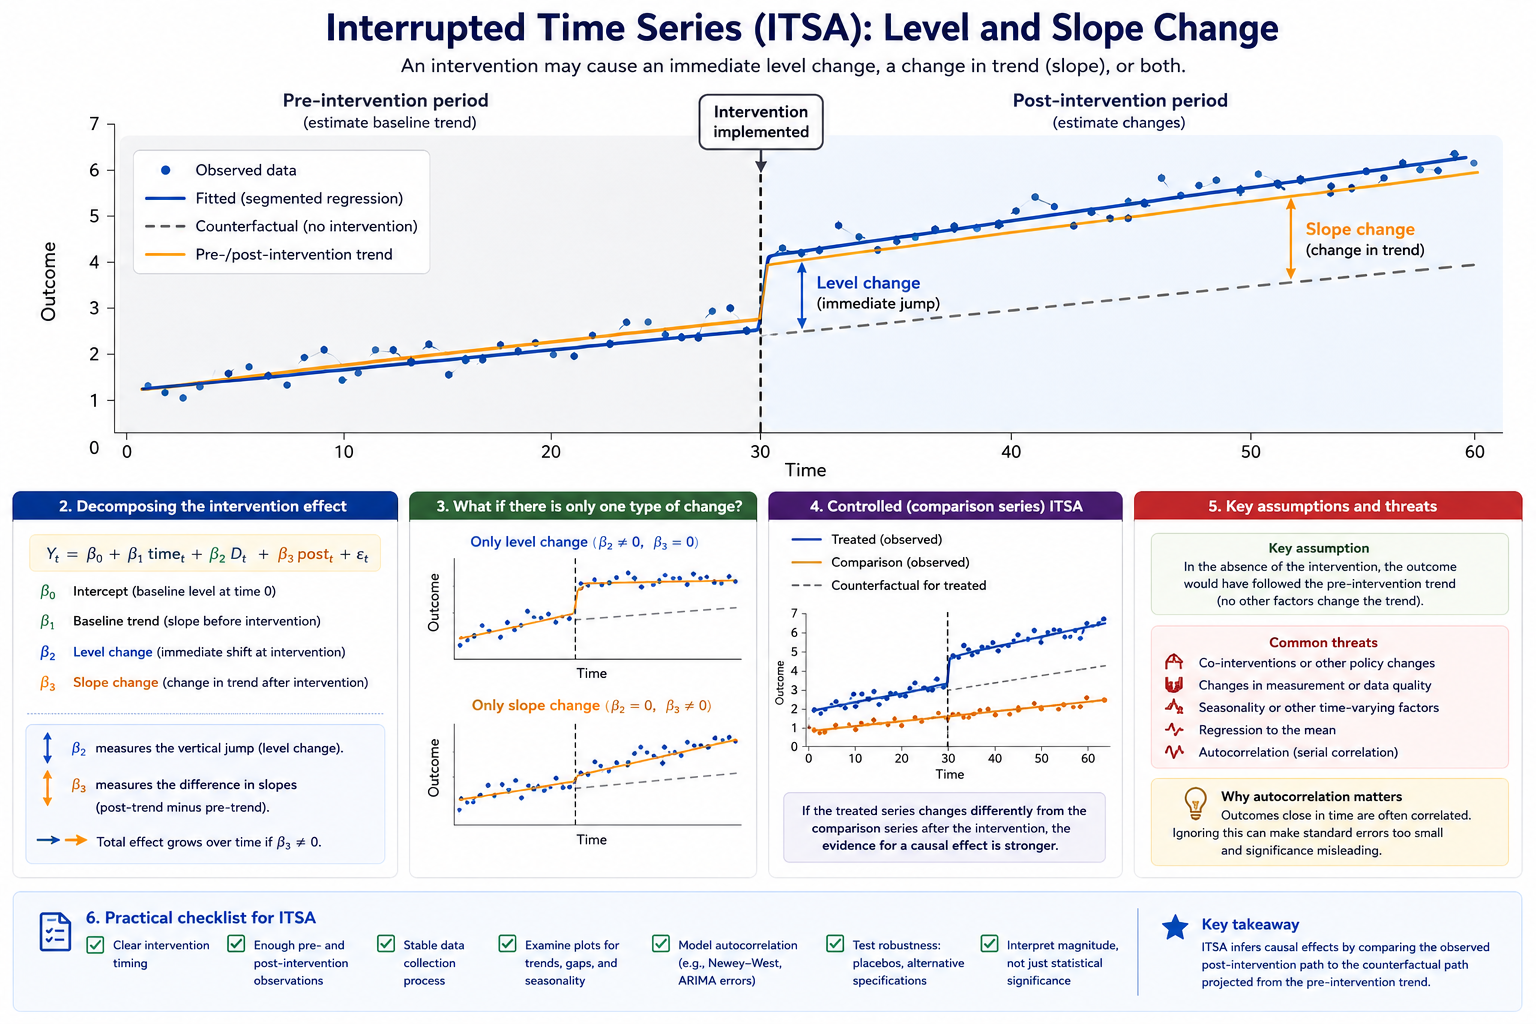
\includegraphics[width=1\linewidth]{images/09_itsa_level_slope} 

}

\caption{Interrupted time series showing an intervention point, observed post-intervention outcomes, and the projected counterfactual trend. The figure illustrates both an immediate level change and a post-intervention slope change, which correspond directly to segmented regression parameters.}\label{fig:fig-itsa-level-slope}
\end{figure}

Figure \ref{fig:fig-itsa-level-slope} illustrates the core logic of interrupted time series analysis. The dashed vertical line marks the intervention point. The dashed counterfactual continuation represents the trajectory that would have been expected if the intervention had not occurred, assuming the pre-intervention trend continued unchanged.

The observed post-intervention series deviates from this projected trend in two important ways. First, there is an immediate jump at the intervention point, known as a \emph{level change}. Second, the long-run trajectory after intervention differs from the original slope, creating a \emph{slope change}. Some policies produce abrupt discontinuities, while others gradually alter the direction or rate of change over time.

Unlike simple before-after comparisons, ITSA explicitly accounts for pre-existing trends. This is one of the main reasons interrupted time series designs are often more credible than simple pre/post analyses.

\section{Counterfactual trends and segmented regression}\label{counterfactual-trends-and-segmented-regression}

The strength of ITSA comes from its use of the historical trend as a counterfactual benchmark. Rather than asking only whether outcomes changed after intervention, ITSA asks whether outcomes changed \emph{more than would have been expected based on prior trajectory}.

Segmented regression is commonly used to estimate these effects statistically. A basic segmented regression model includes:
- a baseline trend before intervention;
- an indicator for the intervention period that estimates the immediate level change; and
- a post-intervention time trend that estimates slope change after intervention.

Figure \ref{fig:fig-itsa-level-slope} maps these concepts visually onto the segmented regression framework. The immediate vertical jump corresponds to the intervention indicator, while the divergence between the post-intervention trend and the projected counterfactual reflects the slope-change parameter.

The following template illustrates a standard ITSA workflow using segmented regression.

\begin{Shaded}
\begin{Highlighting}[]
\CommentTok{\# Template: segmented regression for ITSA}
\CommentTok{\# t0 = the time index where the intervention starts}

\FunctionTok{set.seed}\NormalTok{(}\DecValTok{1}\NormalTok{)}

\NormalTok{n }\OtherTok{\textless{}{-}} \DecValTok{60}
\NormalTok{t0 }\OtherTok{\textless{}{-}} \DecValTok{31}

\NormalTok{df }\OtherTok{\textless{}{-}} \FunctionTok{data.frame}\NormalTok{(}
  \AttributeTok{time =} \DecValTok{1}\SpecialCharTok{:}\NormalTok{n}
\NormalTok{)}

\CommentTok{\# Intervention indicator}
\NormalTok{df}\SpecialCharTok{$}\NormalTok{intervention }\OtherTok{\textless{}{-}} \FunctionTok{ifelse}\NormalTok{(df}\SpecialCharTok{$}\NormalTok{time }\SpecialCharTok{\textgreater{}=}\NormalTok{ t0, }\DecValTok{1}\NormalTok{, }\DecValTok{0}\NormalTok{)}

\CommentTok{\# Time after intervention}
\NormalTok{df}\SpecialCharTok{$}\NormalTok{post\_time }\OtherTok{\textless{}{-}} \FunctionTok{pmax}\NormalTok{(}\DecValTok{0}\NormalTok{, df}\SpecialCharTok{$}\NormalTok{time }\SpecialCharTok{{-}}\NormalTok{ t0 }\SpecialCharTok{+} \DecValTok{1}\NormalTok{)}

\CommentTok{\# Simulated outcome:}
\CommentTok{\# baseline trend + level change + slope change}
\NormalTok{df}\SpecialCharTok{$}\NormalTok{outcome }\OtherTok{\textless{}{-}} \DecValTok{10} \SpecialCharTok{+}
  \FloatTok{0.10} \SpecialCharTok{*}\NormalTok{ df}\SpecialCharTok{$}\NormalTok{time }\SpecialCharTok{+}
  \DecValTok{2} \SpecialCharTok{*}\NormalTok{ df}\SpecialCharTok{$}\NormalTok{intervention }\SpecialCharTok{+}
  \FloatTok{0.05} \SpecialCharTok{*}\NormalTok{ df}\SpecialCharTok{$}\NormalTok{post\_time }\SpecialCharTok{+}
  \FunctionTok{rnorm}\NormalTok{(n, }\DecValTok{0}\NormalTok{, }\FloatTok{0.5}\NormalTok{)}

\CommentTok{\# Segmented regression model}
\NormalTok{model\_itsa }\OtherTok{\textless{}{-}} \FunctionTok{lm}\NormalTok{(}
\NormalTok{  outcome }\SpecialCharTok{\textasciitilde{}}\NormalTok{ time }\SpecialCharTok{+}\NormalTok{ intervention }\SpecialCharTok{+}\NormalTok{ post\_time,}
  \AttributeTok{data =}\NormalTok{ df}
\NormalTok{)}

\FunctionTok{summary}\NormalTok{(model\_itsa)}

\CommentTok{\# Interpretation:}
\CommentTok{\# {-} intervention = immediate level change}
\CommentTok{\# {-} post\_time    = slope change after intervention}
\end{Highlighting}
\end{Shaded}

In practice, interpretation should always be guided by the intervention's theory of change. Some interventions are expected to create immediate discontinuities, while others may influence outcomes gradually over time.

For example, a media campaign may have delayed behavioural effects, whereas a tax increase may alter prices immediately.

\section{Assumptions and threats to validity}\label{assumptions-and-threats-to-validity}

The most important assumption in ITSA is that the pre-intervention trend would have continued in the absence of intervention. In other words, the projected counterfactual trend must be a reasonable approximation of what would have happened without policy change.

Several threats can weaken this assumption.

One major threat is the presence of \emph{co-interventions}, where another policy or event occurs around the same time as the intervention. If multiple changes occur simultaneously, separating their effects becomes difficult.

Changes in data collection, reporting systems, or measurement definitions may also create artificial discontinuities that resemble intervention effects.

Seasonality is another important issue. Many economic, environmental, and health outcomes fluctuate systematically across months, quarters, or seasons. Ignoring these recurring patterns may bias intervention estimates.

Regression to the mean can also create misleading patterns when interventions are implemented after unusually high or low observations.

Importantly, interrupted time series data frequently exhibit \emph{autocorrelation}, meaning nearby observations remain statistically dependent across time. Ignoring autocorrelation may produce standard errors that are too small and statistical significance that appears stronger than it truly is.

For this reason, ITSA often requires specialized error structures or time-series corrections beyond ordinary least squares assumptions.

Reliable ITSA also requires sufficient observations before and after intervention. Too few pre-intervention observations make it difficult to establish whether the baseline trend is stable, while too few post-intervention observations may obscure gradual slope changes.

\section{Extensions and practical applications}\label{extensions-and-practical-applications}

Interrupted time series analysis can be extended in several important ways.

Researchers may include additional covariates to adjust for changing contextual factors. Seasonal terms can account for repeating cyclical patterns, while autoregressive error structures can address autocorrelation directly.

One particularly important extension is \emph{controlled interrupted time series analysis}, where a comparison series unaffected by the intervention is included alongside the treated series. Comparison groups help distinguish intervention effects from broader system-wide changes occurring at the same time.

Interaction terms may also be used to evaluate heterogeneous effects across regions, demographic groups, or institutions.

In applied policy analysis, ITSA is frequently used in:
- public health evaluation,
- pharmaceutical policy,
- environmental regulation,
- healthcare utilization studies,
- transportation safety,
- and education reform.

Because many large-scale policies are implemented at clearly identifiable dates, interrupted time series designs are often highly practical in real-world evaluation settings.

\section{Common pitfalls and key takeaways}\label{common-pitfalls-and-key-takeaways-5}

Several recurring mistakes can weaken interrupted time series analysis. One common problem is declaring causal effects without evaluating whether other simultaneous events may explain the observed change. Another is relying on very short pre-intervention periods that provide little evidence regarding baseline stability.

Researchers may also ignore autocorrelation, seasonality, or structural breaks, leading to overly confident statistical inference.

Importantly, ITSA should not be interpreted as a purely mechanical statistical procedure. Credible interpretation depends on institutional knowledge, policy timing, implementation details, and the plausibility of the counterfactual trend assumption.

Overall, interrupted time series analysis is one of the most powerful quasi-experimental tools available when interventions occur at identifiable points in time and stable pre-intervention trends exist. By explicitly modeling counterfactual trajectories, ITSA provides a structured framework for evaluating policy effects in settings where randomization is impractical or impossible.

\chapter{Interrupted Time Series Analysis (ITSA): Worked Workflow}\label{itsa-applied}

This chapter summarizes a practical workflow for implementing ITSA. The goal is to structure applied work so that assumptions are checked, diagnostics are reported, and results are communicated clearly.

Roadmap

We outline a step-by-step process from data preparation to model refinement and reporting. The workflow is compatible with regression-based ITSA and time-series error models.

Learning objectives

\begin{itemize}
\tightlist
\item
  Prepare and structure time-series data for ITSA.
\item
  Use plots to check trends, outliers, and seasonality.
\item
  Specify a segmented regression model and interpret parameters.
\item
  Diagnose autocorrelation and adjust inference.
\item
  Report results with uncertainty and sensitivity checks.
\end{itemize}

\begin{figure}

{\centering 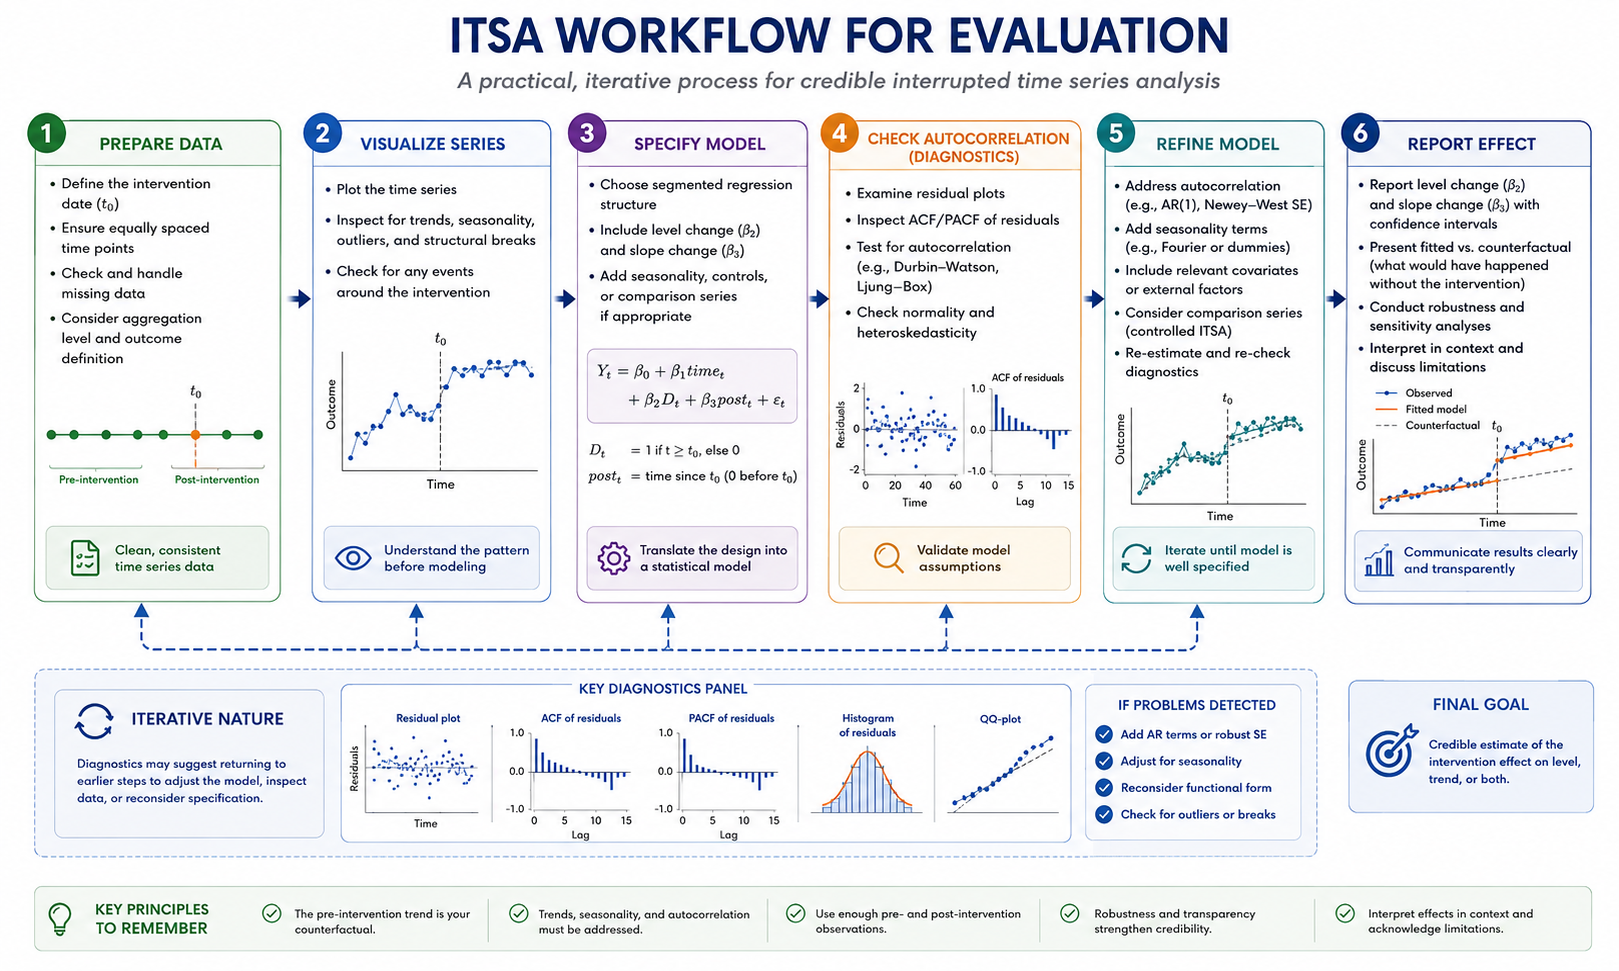
\includegraphics[width=0.95\linewidth]{images/10_itsa_workflow} 

}

\caption{Practical ITSA workflow: prepare data, visualize, specify model, check autocorrelation, refine, and report effects with uncertainty and sensitivity checks.}\label{fig:fig-itsa-workflow}
\end{figure}

Figure \ref{fig:fig-itsa-workflow} is a checklist for applied work. It helps ensure that evaluation is transparent and reproducible.

After fitting a segmented regression, a key check is whether residuals are autocorrelated.

\begin{Shaded}
\begin{Highlighting}[]
\CommentTok{\# Template: basic diagnostics after a segmented regression}
\CommentTok{\# install.packages(c("lmtest","sandwich","forecast")) if needed}

\FunctionTok{library}\NormalTok{(lmtest)}
\FunctionTok{library}\NormalTok{(forecast)}

\CommentTok{\# model\_itsa is the fitted model from the segmented regression}
\FunctionTok{dwtest}\NormalTok{(model\_itsa)                 }\CommentTok{\# Durbin{-}Watson test for autocorrelation}
\FunctionTok{checkresiduals}\NormalTok{(model\_itsa)         }\CommentTok{\# residual plot + ACF check}
\end{Highlighting}
\end{Shaded}

\section{Reporting recommendations}\label{reporting-recommendations}

A strong ITSA report includes:

\begin{itemize}
\tightlist
\item
  clear definition of the intervention and timing
\item
  justification for pre and post windows
\item
  plots of the outcome with intervention markers
\item
  model specification with level and slope terms
\item
  autocorrelation diagnostics and corrected inference
\item
  sensitivity analysis (alternative windows, functional forms, seasonality)
\end{itemize}

Common pitfalls

\begin{itemize}
\tightlist
\item
  Reporting a single model with no sensitivity checks.
\item
  Omitting diagnostic evidence for autocorrelation.
\item
  Over-interpreting short post-intervention windows.
\end{itemize}

Key takeaways

\begin{itemize}
\tightlist
\item
  A transparent workflow improves credibility.
\item
  Sensitivity checks are part of good evaluation practice.
\end{itemize}

\end{document}
